%gji_extra_guide.tex
% \documentclass[extra,mreferee]{gji}
% \usepackage{mathrsfs,amsmath}
% \usepackage{timet}

\documentclass[a4paper, 11pt]{article}
\usepackage[pdftex]{graphicx}
\usepackage{fullpage}
\usepackage{mathrsfs, amsmath, amsfonts}
\usepackage{framed, color, fancybox}

\author{Seogi Kang and Douglas W. Oldenburg}  
\title{On recovering distributed IP information in inductive source time domain electromagnetic data} 


%% =============================================================================
%% My equations
%% =============================================================================

\renewcommand{\div}{\nabla\cdot}
\newcommand{\grad}{\vec \nabla}
\newcommand{\curl}{{\vec \nabla}\times}
\newcommand {\J}{{\vec J}}
\renewcommand{\H}{{\vec H}}
\newcommand {\E}{{\vec E}}
\newcommand{\siginf}{\sigma_\infty}
\newcommand{\dsig}{\triangle\sigma}
\newcommand{\dcurl}{{\mathbf C}}
\newcommand{\dgrad}{{\mathbf G}}
\newcommand{\Acf}{{\mathbf A_c^f}}
\newcommand{\Ace}{{\mathbf A_c^e}}
\renewcommand{\S}{{\mathbf \Sigma}}
\newcommand{\St}{{\mathbf \Sigma_\tau}}
\newcommand{\T}{{\mathbf T}}
\newcommand{\Tt}{{\mathbf T_\tau}}
\newcommand{\diag}{\mathbf{diag}}
\newcommand{\M}{{\mathbf M}}
\newcommand{\MfMui}{{\M^f_{\mu^{-1}}}}
\newcommand{\MfMuoi}{{\M^f_{\mu_0^{-1}}}}
\newcommand{\dMfMuI}{{d_m (\M^f_{\mu^{-1}})^{-1}}}
\newcommand{\dMfMuoI}{{d_m (\M^f_{\mu_0^{-1}})^{-1}}}
\newcommand{\MeSig}{{\M^e_\sigma}}
\newcommand{\MeSigInf}{{\M^e_{\sigma_\infty}}}
\newcommand{\MeSigInfEtab}{{\M^e_{\sigma_\infty \bar{\eta}}}}
\newcommand{\MeSigInfEtat}{{\M^e_{\sigma_\infty \peta}}}
\newcommand{\MedSig}{{\M^e_{\triangle\sigma}}}
\newcommand{\MeSigO}{{\M^e_{\sigma_0}}}
\newcommand{\Me}{{\M^e}}
\newcommand{\Js}{\mathbf{J}^s}
\newcommand{\Mes}[1]{{\M^e_{#1}}}
\newcommand{\Mee}{{\M^e_e}}
\newcommand{\Mej}{{\M^e_j}}
\newcommand{\BigO}[1]{\mathcal{O}\bigl(#1\bigr)}
\newcommand{\bE}{\mathbf{E}}
\newcommand{\bEp}{\mathbf{E}^p}
\newcommand{\bB}{\mathbf{B}}
\newcommand{\bBp}{\mathbf{B}^p}
\newcommand{\bEs}{\mathbf{E}^s}
\newcommand{\bBs}{\mathbf{B}^s}
\newcommand{\bH}{\mathbf{H}}
\newcommand{\B}{\vec{B}}
\newcommand{\D}{\vec{D}}
\renewcommand{\H}{\vec{H}}
\newcommand{\s}{\vec{s}}
\newcommand{\bfJ}{\bf{J}}
\newcommand{\vecm}{\vec m}
\renewcommand{\Re}{\mathsf{Re}}
\renewcommand{\Im}{\mathsf{Im}}
\renewcommand {\j}  { {\vec j} }
\newcommand {\h}  { {\vec h} }
\renewcommand {\b}  { {\vec b} }
\newcommand {\e}  { {\vec e} }
\renewcommand {\d}  { {\vec d} }
\renewcommand {\u}  { {\vec u} }

\renewcommand {\dj}  { {\mathbf{j} } }
\renewcommand {\dh}  { {\mathbf{h} } }
\newcommand {\db}  { {\mathbf{b} } }
\newcommand {\de}  { {\mathbf{e} } }

\newcommand{\vol}{\mathbf{v}}
\newcommand{\I}{\vec{I}}
\newcommand{\A}{\mathbf{A}}
\newcommand{\bI}{\mathbf{I}}
\newcommand{\bus}{\mathbf{u}^s}
\newcommand{\brhss}{\mathbf{rhs}_s}
\newcommand{\bup}{\mathbf{u}^p}
\newcommand{\brhs}{\mathbf{rhs}}
%%-------------------------------
\newcommand{\bon}{b^{on}(t)}
\newcommand{\bp}{b^{p}}
\newcommand{\dbondt}{\frac{db^{on}(t)}{dt}}
\newcommand{\dfdt}{\frac{df(t)}{dt}}
\newcommand{\dfdtdsiginf}{\frac{\partial\frac{df(t)}{dt}}{\partial\siginf}}
\newcommand{\dfdsiginf}{\frac{\partial f(t)}{\partial\siginf}}
\newcommand{\dbgdsiginf}{\frac{\partial b^{Impulse}(t)}{\partial\siginf}}
\newcommand{\digint}{\frac{2}{\pi}\int_0^{\infty}}
\newcommand{\Gbiot}{\mathbf{G}_{Biot}}
%%-------------------------------
\newcommand{\peta}{\tilde{\eta}}
\newcommand{\eFmax}{\e^{\ F}_{max}}
\newcommand{\eref}{\e^{\ ref}}
\newcommand{\jref}{\j^{\ ref}}
\newcommand{\dip}{d^{IP}}
\newcommand{\sigpert}{\delta\sigma}
\newcommand{\bzip}{b_z^{IP}}
\newcommand{\dbzdtip}{\frac{\partial b_z^{IP}}{\partial t}}

%% =============================================================================
%% End of my equations
%% =============================================================================


% \title[] {On recovering distributed IP information in airborne time domain electromagnetic data} 
% \author[] {Seogi Kang and Douglas W. Oldenburg}  
% \newcommand{\btx}{\textsc{BibTeX}}

\begin{document}
\maketitle
\tableofcontents
\clearpage

\section{Introduction}
The electrical conductivity of earth materials can be frequency dependent with the effective conductivity decreasing with decreasing frequency due to the buildup of electric charges that occur under the application of an electric field.
Effectively, the rock is electrically polarized. Finding this induced polarization (IP) response has been important in mineral exploration but it is also important in environmental problems, groundwater flow, and site characterization. 
Polarization charges can accumulate whenever there is an electric field in a medium and so the transmitter can be a galvanic or inductive source. 
Different excitation mechanisms originated from these two different sources, makes a principal difference in IP effects. 
Since the inductive source is divergence-free it does not have any steady-state electric field, whereas galvanic source has one. 
Understanding of IP effects for the galvanic source has been well-established for several decades (\cite{seigel1959}, \cite{seigel1974}): electrical IP (EIP). Especially for the restoration of the chargeability, linearized kernel function has been used assuming no EM induction effects (\cite{doug1994}). For the inductive source IP (ISIP), similar linearized approach to recover 3D IP information has been investigated in the frequency domain data (\cite{Marchant2012b}). However, recovering 3D IP information from the time domain EM (TEM) data, has not been carefully studied. 
Our focus in this article is upon the potential for extracting IP information from inductive source TEM systems such as the coincident loop instrument for airborne TEM (ATEM) survey. The observed data for this system often have negative transients (\cite{Kratzer2012} add Mt Milligan, TKC). \cite{Weidelt1982} showed that the most plausible explanation of these is that they are caused by IP effects. 

To extract distributed IP information from the inductive source TEM data, we use similar linearized inversion approach (\cite{seigel1959,doug1994}), which has extensively been used in the industry. Application of this to our case will include three principal steps: 1) Restoration of the 3D conductivity, 2) EM decoupling, and 3) 3D IP inversion with linearized kernel function. 
The first step is not trivial because the observed TEM data can be contaminated by IP effect. 
Accordingly, the recovered conductivity may have some discrepancy with the true one.
The IP response computed from the second step may include some residual field due to this incorrect conductivity. 
Effect of this incorrect conductivity to our inversion procedure should be investigated. 
Linearization of IP responses for the inductie source TEM data, and its validation can be an essential factor to perform the 3D IP inversion. 
Here the difference of the IP response on the inductive source from the galvanic source should be carefully incorporated into the linearized kernel.  

To demonstrate a 3D IP inversion procedure to recover distributed IP information from the TEM data, in this article, we first define IP datum by decomposing the observed EM response. 
Based on this, then we derive a linearized kernel of IP responses for the TEM data. 
Next, we suggest a 3D IP inversion methodology to recover multiple time channels of the pseudo-chargeability, and also investigate a potential to extract intrinsic Cole-Cole parameters from pseusdo-chargeability. Finally, we carefully analyze and validate each step of our 3D IP inversion procedure with numerical examples of ATEM survey.       
    
%% =============================================================================
%% Section. Complex conductivity
%% =============================================================================

\section{Complex conductivity}
An often-used representation for complex conductivity in the frequency domain is the Cole-Cole model \cite{COLE}:
\begin{equation}
  \sigma(\omega) = \sigma_{\infty} - \sigma_{\infty}\frac{\eta}{1+(1-\eta)(\imath\omega\tau)^c} = \sigma_{\infty} + \triangle\sigma(\omega),
  \label{eq: sigma_freq}
\end{equation}
where $\sigma_{\infty}$ is the conductivity at infinite frequency, $\eta$ is the intrinsic chareability, $\tau$ is the time constant and $c$ is the frequency dependency. Real and imaginary parts of complex conductivity in frequency domain are shown in Figure ~\ref{Fig:FDandTDCole}(a) with Cole-Cole parameters: $\siginf$ = $10^{-2}$ S/m, $\eta $ = 0.5, $\tau$ = 0.01 and $c$=1. By applying inverse Fourier transform with time dependency, $e^{\imath\omega t}$, we have
\begin{equation}
  \sigma(t) = \mathscr{F}^{-1}[\sigma(\omega)] = \sigma_{\infty}\delta(t) + \triangle\sigma(t),
  \label{eq: sigma_time}
\end{equation}
where $\delta(t)$ is Dirac delta function and $\mathscr{F}^{-1}[\cdot]$ is inverse Fourier transform operator. 
We rewrite $\dsig(t)$ as 
\begin{equation}
  \dsig(t) = - \siginf\peta^{I}(t),
  \label{eq: sigma_time_c1}
\end{equation}
where intrinsic pseudo-chargeability, $\peta^{I}(t)$ is
\begin{equation}
    \peta^{I}(t) = -\frac{\dsig(t)}{\siginf}. %=\frac{\eta}{(1-\eta)\tau}e^{-\frac{t}{(1-\eta)\tau}}u(t)
    \label{eq: intrinsic_peta}
\end{equation}
Cole-Cole model in time domain is also shown in Figure ~\ref{Fig:FDandTDCole}(b). Used Cole-Cole parameters here are same as the above.

\begin{figure}
  \centering
  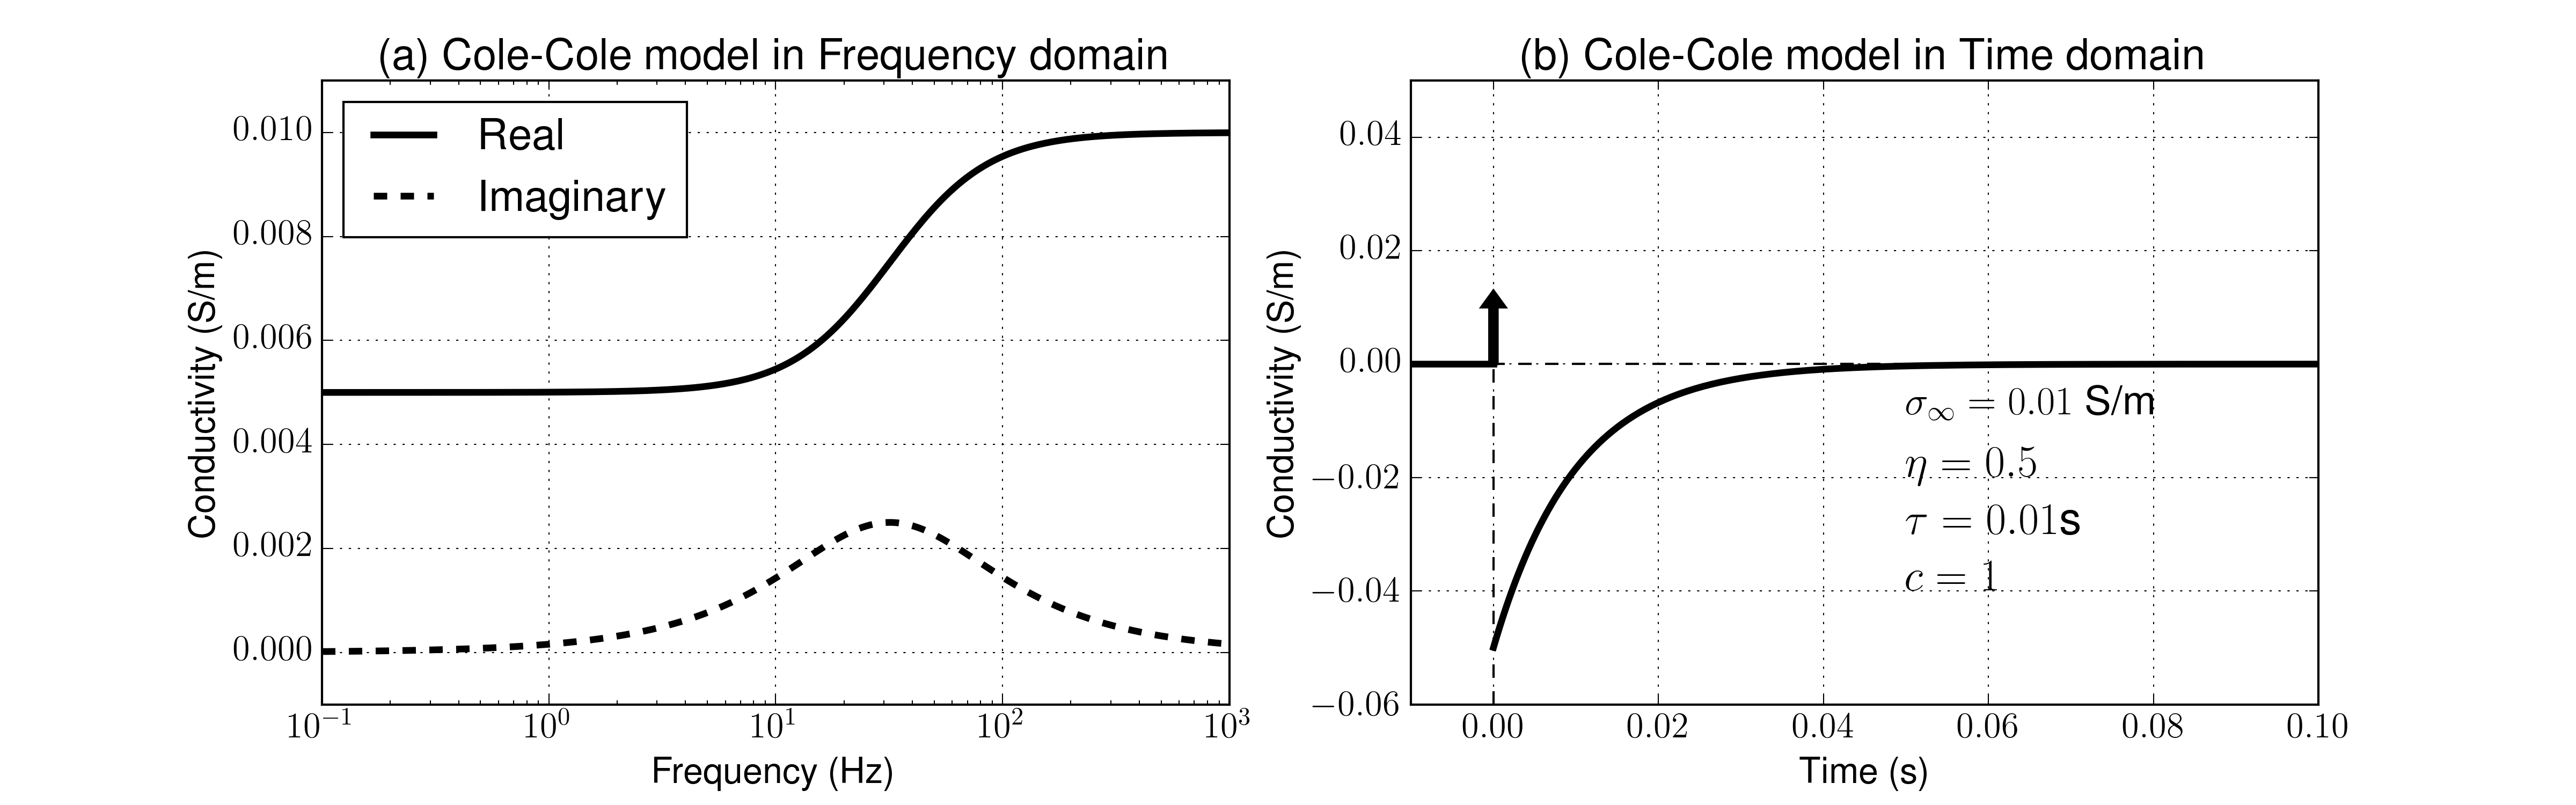
\includegraphics[width=1.0\textwidth]{figures/FDandTDCole.png}
  \caption{Cole-Cole model in frequency domain (a) and time (b) domain. }
  \label{Fig:FDandTDCole}
\end{figure}

%% =============================================================================
%% Section. Decomposition of EM responses
%% =============================================================================

\section{Decomposition of observed responses}
IP effect in the observed data is coupled with EM effect. We decompose these two effects in the observation. 
Consider Maxwell's equations in time domain:
\begin{equation}
  \curl{\e} = -\frac{\partial \b}{\partial t}
  \label{eq: total_farad}
\end{equation}
\begin{equation}
  \curl{\frac{1}{\mu}\b} - \j= \j_{s},
  \label{eq: total_coulomb}
\end{equation}
where $\e$ is the electric field ($V/m$), $\b$ is the magnetic flux density ($Wb/m^2$) and $\mu$ is the magnetic permeability ($H/m$). Here $\j$ is the conduction current. In the frequency domain the current density $\J$ is related to conductivity via $\J(\omega) = \sigma(\omega)\E(\omega)$ where $\E$ is the electric field.
Converting this relationship to time domain using inverse Fourier transform yields:
\begin{equation}
  \j(t) = \sigma(t)\otimes \e(t),
  \label{eq: ohmslaw1}
\end{equation}
where $\otimes$ indicates time convolution. 
For causal signals, which is defined when $t \ge 0$, convolution between $a(t)$ and $b(t)$ can be written as
\begin{equation}
  a(t) \otimes b(t) = \int_0^t a(u) b(t-u) du.
  \label{eq: convolution}
\end{equation}
That is the current density depends upon the previous history of the electric field.
As in \cite{Smith1988a}, we let total fields as $\e = \e^{F} + \e^{IP}$, $\b = \b^{F} + \b^{IP}$ and $\j = \j^{F} + \j^{IP}$, where superscript $F$ indicates fundamental and $IP$ is induced polarization. 
Here fundamental fields indicate EM fields without IP effect. 
Substituting into equations (\ref{eq: total_farad}) and (\ref{eq: total_coulomb}) yields the following sequences:
\begin{equation}
  \curl({\e^{F}+\e^{IP}}) = -\frac{\partial}{\partial t} (\b^{F}+\b^{IP}),
\end{equation}
\begin{equation}
  \curl\frac{1}{\mu}(\b^{F}+\b^{IP}) - (\j^{F}+\j^{IP})= \j_{s}.
\end{equation}
By canceling out vectors associated with $EM$ terms, we have
\begin{equation}
  \curl \e^{IP} = -\frac{\partial \b^{IP}}{\partial t},
  \label{eq: eq_secondary_farad}
\end{equation}
\begin{equation}
  \curl{\frac{1}{\mu}\b^{IP}} = \j^{IP}.
  \label{eq: eq_secondary_coulomb}
\end{equation}
In addition, associated $EM$ equations can be written as
\begin{equation}
  \curl \e^{F} = -\frac{\partial \b^{F}}{\partial t},
  \label{eq: eq_primary_farad}
\end{equation}
\begin{equation}
  \curl{\frac{1}{\mu}\b^{F}} -\j^{F} = \j_s.
  \label{eq: eq_primary_coulomb}
\end{equation}
Here
\begin{equation}
  \j^{F} = \siginf\e^{F}.
  \label{eq: jF}
\end{equation}
Let $F[\cdot]$ denote operator associated with Maxwell’s equations and let $d$ denote the observed electromagnetic field thus, this includes both EM and IP effects. Keeping the same notation, we also write $d = d^{F} + \dip$. Therefore, we define IP datum as
\begin{equation}
  \dip = d - d^{F} = F[\sigma(t)]-F[\siginf].
    \label{eq: IPdatum_syn}
\end{equation}
Here $F[\siginf]$ correspond to the fundamental response ($d^F$). 
This subtraction process acts as an EM decoupling process, which reduces the EM effects in the measured responses. 
This formed the basis of work by \cite{routh2001}. 
Therefore, recovering the distribution of $\siginf$ in 3D space, may allow us to identify  IP datum, which are embedded in the observed responses. 

%% =============================================================================
%% Section. Linearization of EM responses
%% =============================================================================

\section{Linearization of EM responses}
A major difference of the inductive source from the galvanic source is the absence of the steady-state electric field. 
This generates a principal difference on the IP response for both inductive and galvanic sources. 
To carefully examine this, we define the IP current ($\j^{IP}$) as
\begin{equation}
  \j^{IP} = \siginf \e^{IP} + \j^{pol},
  \label{eq:IP_current}
\end{equation}
where the polarization current ($\j^{pol}$) is
\begin{equation}
  \j^{pol}(t) = \dsig(t) \otimes \e(t).
  \label{eq:polarization_current}
\end{equation}
The polarization current is the convolution between $\dsig (t)$ and the total electric field. 
Thus, if the electric field has different characteristic for the inductive and galvanic sources, this will be incorporated in the polarization current.
We consider two cases: a) galvanic source without EM induction and b) inductive source with EM induction. The first case corresponds to Electrical IP (EIP; \cite{seigel1959}), and the second one is ISIP.
Figure \ref{F:DCEM_F_current} shows the magnitude of the fundamental electric field ($\e^{F}$) in the earth for those two cases. 
For the galvanic source, the electric field is instantaneous due to the steady-state electric field (Figure \ref{F:DCEM_F_current} (a)). 
However, for the inductive source, the electric field on off-time is not zero, but increases to the peak then decays as shown in Figure \ref{F:DCEM_F_current} (b). 
The polarization current for two different sources will be significantly affected by these different electric fields. 
To capture this difference in the linearized kernel for the IP response, we define pseudo-chargeability ($\peta(t)$) as 
\begin{equation}
  \peta(t) = -\frac{\j^{pol}(t)}{\j^{\ ref}},
  \label{eq:pseudochargeability_0}
\end{equation}
where the reference current ($\j^{ref}$) is defined as 
\begin{equation}
  \j^{\ ref} = \siginf \eref.
  \label{eq:reference_current}
\end{equation}
Here $\eref$ is the reference electric field. 
Both $\j^{\ ref}$ and $\eref$ are static field that is independent on time. 
The pseudo-chargeability is the fraction of the polarization current and the reference current. From the definition of the polarization current, we can simply expect magnitude of the IP response is proportional to that of the pseudo-chargeability, and it varies in time. 
Becase we linearize IP response as a function of the pseudo chargeability, this can be one of the most important property in our linearization. 
To evaluate the pseudo-chargeability, we have to identify the reference current or electric fields. 
For the EIP case, the choice of the reference current is obvious because the electric field is independent on time without IP effect as shown in Figure \ref{F:DCEM_F_current}(a). 
Natural choice of the reference electric field in this case may be the fundamental electric field at any on-time. 
For the inductive source, the electric field does not reach to the steady-state, but increases to the peak then decreases. 
Thus an intuitive choice of the reference electric field can be the maximum of the $\e^{F}$. 
And this time when the maximum electric field occurs can be considered as the reference time ($t^{\ ref}$)
This reference electric field ($\eref$) and the reference time are going to be different in each pixel of the earth. 
Accordingly, both $\eref$ and $t^{\ ref}$ have 3D distribution. 
For both EIP and ISIP cases, we mathematically present our choice of the reference field as
\begin{equation}
  \eref = \e^{F}(t) \otimes \delta(t-t^{\ ref}). 
  \label{eq:reference_electricfield}
\end{equation}
The reference time for the EIP case can be arbitrary on-time, because the fundamental electric field for the EIP case is independent on time. 

By rearranging equation (\ref{eq: pseudochargeability_equivalent}), we obtain 
\begin{equation}
  \j^{pol} = -\jref\peta(t). 
  \label{eq:polarization_current_concept}
\end{equation}
Baed on this, we form a conceptual model that the polarization current has opposite direction to the reference current, and proportional to the pseudo-chargeability ($\peta(t)$). 
This reveresed direction of the polarization current to the reference current can be a direct reason why the ATEM data show negative trasients with the IP effect. 
This conceptual model about the polarization current shown in equation(\ref{eq:polarization_current_concept}) is consistent with \cite{seigel1959}'s result. 
\begin{figure}
  \centering  
  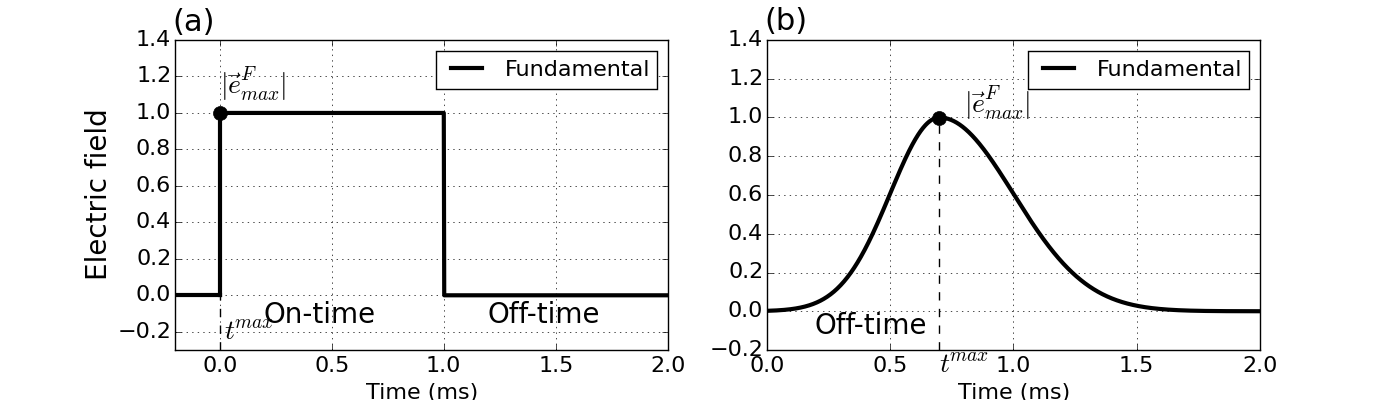
\includegraphics[width=1.0\textwidth]{figures/DCEM_F_current.png}
  \caption{Conceptual diagram for the amplitude of the fundamental electric fields. (a) EIP and (b) ISIP cases.}
  \label{F:DCEM_F_current}
\end{figure}
  

%% =============================================================================
%% Sub-Section. Linearization 

\subsection{Linearization}
Our goal of the linearization is to express IP response ($\dip$) as a function of the pseudo-chargeability $(\peta(t))$ in time. 
Therefore, we need obtain a form of linear equation like $\dip(t) = J[\peta(t)]$, where $J[\cdot]$ is a linear operator, which is independent on time. 

For the general use of the linearzied IP responses in various TEM surveys, we consider a general EM system, which can be either galvanic and inductive sources. 
Let the total electric field, $\e(t)$ can be approximated as
\begin{equation}
  \e(t) \approx \eref w^e(t),
  \label{eq: e_with_eref}
\end{equation}
where $w^e(t)$ is defined as:
\begin{equation}
  w^e(t) = \left\{ 
  \begin{array}{l l}
    w^{ref}(t) & w^{ref}(t) \ge 0 \\
    0 & \text{if } w^{ref}(t) < 0, 
  \end{array}\right.
  \label{eq: we}
\end{equation}
with
\begin{equation}
  w^{ref}(t) = \frac{\e^F(t)\cdot\eref}{\eref\cdot\eref}.
  % \label{eq: we}
\end{equation}
Here $w^{ref}(t)$ is a dimensionless function that prescribes the time history of the electric field at each location and the reference electric field ($\eref$) is an appropriate scaling for the electric field, which is independent on time. 
This indicates that the direction of the electric field does not change in time. 
In addition, by the definition of $w^e(t)$, we projects negatives values of  $w^{ref}(t)$ to zero.
This projection is based on the conceptual model that the polarization current has opposite direction to the reference current (equation (\ref{eq:polarization_current_concept})). 
% Note that this assumption is only applied to the second term on right-hand side of equation (\ref{eq:IP_current}). 

Substituting this into equation (\ref{eq:IP_current}) yields
\begin{eqnarray*}
  \j^{IP}(t) \approx \siginf\e^{IP}(t) + \frac{\dsig(t)\otimes w^e(t)}{\siginf}\j^{\ ref},
\end{eqnarray*}
where the reference current density is defined as
\begin{equation}
  \j^{ref} = \siginf\eref.
\end{equation}
Letting pseudo-chargeability as
\begin{equation}
    \peta(t) = -\frac{\dsig(t)\otimes w^e(t)}{\siginf} \approx -\frac{\j^{pol}(t)}{\j^{\ ref}},
    \label{eq: pseudochargeability}
\end{equation}
we obtain
\begin{eqnarray}
  \j^{IP}(t) = \siginf\e^{IP}(t) + \j^{pol}(t) \approx \siginf\e^{IP}(t) -\j^{\ ref}\peta(t).
  \label{eq: jip_EMIP}
\end{eqnarray}
Because the reference current is static, any time-dependency in the pseudo-chargeability is originated from the polarization current. 

Using Helmholtz decomposition, $\e$ can be decomposed as $\e=-\vec{a}-\grad\phi$, where $\vec{a}$ and $\phi$ is electric vector and scalar potentials, respectively and $\div\vec{a}=0$. Physically, those two terms indicate charge-build up and EM induction effects, which induce galvanic and vortex currents, respectively. So, $\e^{IP}$ can be decomposed as
\begin{equation}
  \e^{IP}=-\vec{a}^{IP}-\grad\phi^{IP}.
  \label{eq: eip_helmholtz}
\end{equation}
Now we make another assumption:
\begin{equation}
  \e^{IP} \approx  \e^{IP}_{approx} = -\grad\phi^{IP},
  \label{eq: eip_approx}
\end{equation}
which means $\e^{IP}$ term in equation (\ref{eq: jip_EMIP}) is dominated by galvanic effect ($\frac{\partial\b^{IP}}{\partial t}\approx 0$). First taking $\div$ to equation (\ref{eq: jip_EMIP}) then by substituting  $\e^{IP}$ with equation (\ref{eq: eip_approx}) with some linear algebra, we obtain
\begin{equation}
  \phi^{IP}(t) \approx -[\div \siginf\grad]^{-1}\div\j^{\ ref}\peta(t).
  \label{eq: phiIPapprox_general}
\end{equation}
By taking $\grad$ to this equation, we obtain 
\begin{equation}
    \e^{IP}_{approx} = \grad[\div \siginf\grad]^{-1}\div\j^{\ ref}\peta(t).
    \label{eq: eip_approx_full}
\end{equation}
Thus, the electric field due to the IP effect can be expressed as a function of $\peta(t)$ in time. This can be applicable to EIP case.   
The type of the data for the inductive source is often either $\b$ or $\frac{\partial \b}{\partial t}$ thus, we also need to compute $\b^{IP}$ or $\frac{\partial \b^{IP}}{\partial t}$.
For this, we first compute $\j^{IP}$ then use Biot-Savart law to compute $\b^{IP}$ or $\frac{\partial \b^{IP}}{\partial t}$. 
Substituting equation (\ref{eq: phiIPapprox_general}) into equation (\ref{eq: jip_EMIP}), approximated IP current density, $\j^{IP}_{approx}$ can be expressed as
\begin{equation}
  \j^{IP}(t) \approx \j^{IP}_{approx} = \bar{S}\siginf\eref\peta(t),
  \label{eq: jip_approx}
\end{equation}
where
\begin{equation}
  \bar{S} = -\Big(-\siginf\grad[\div \siginf\grad]^{-1}\div+\bar{I}\Big)
\end{equation}
and $\bar{I}$ is an identity tensor. Then by using Biot-Savart law we have:
\begin{equation}
  \b^{IP}_{approx}(\vec{r}; t) = \frac{\mu_0}{4\pi}\int_{\Omega}  \frac{\bar{S}\eref(\vec{r}_s)\times\hat{r}}{|\vec{r}-\vec{r}_s|^2}\peta(t)d\vec{r}_s.
  \label{eq: BiotbIP_approx}
\end{equation}
By taking time derivative to the above equation we have
\begin{equation}
  -\frac{\partial\b^{IP}_{approx}}{\partial t}(\vec{r}; t) = \frac{\mu_0}{4\pi} \int_{\Omega}  \frac{\bar{S}\eref(\vec{r}_s)\times\hat{r}}{|\vec{r}-\vec{r}_s|^2} \Big( -\frac{\partial \peta(t)}{\partial t} \Big) d\vec{r}_s.
  \label{eq: BiotbIPdt_approx}
\end{equation}
Here we set $-\frac{\partial \b^{IP}_{approx}}{\partial t}$ as our IP datum, to keep the sign of the IP response as negative. 
Accordingly, the input of the kernel is determined to $-\frac{\partial \peta(t)}{\partial t}$. 
Various types of the IP fields shown in equations (\ref{eq: eip_approx_full}), (\ref{eq: BiotbIP_approx}) and (\ref{eq: BiotbIPdt_approx}) are function of $\peta(t)$.
The time dependency only rises from $\peta(t)$. 
To summarize, with two main assumptions: a) $\e^{IP}\approx -\grad\phi^{IP}$ and b) $\e \approx \e^{ref}w^e(t)$, we show that IP fields can have linear relationship with $\peta(t)$. 

Therefore, $\dip$ responses, which can be various types of electromagnetic fields, can be represented as $\dip(t) = J[\peta(t)]$ for both inductive and galvanic sources. In discretized space this can be expressed as
\begin{equation}
  \mathbf{d}^{IP}_i = \mathbf{J}\peta_i,
  \label{eq: dIP_lineareq}
\end{equation}
where $\mathbf{J}$ is corresponding sensitivity matrix and the subscript $i$ indicates $i^{th}$ time channel. 
Boldface of upper and lower cases indicate a matrix and column vector in discretized space. 
Detailed description for the discretization of the linearized kernel is shown in sections \ref{section:maxwell_discrete} and \ref{section:linearkernel_discrete}. 
This linear equation will be a forward kernel for the 3D IP inversion. 
Our forward kernel has capability to handle different types of electromagnetic fields, thus this has some potential to be used in different types of TEM surveys. 
On the other hand, the assumptions that we have made to formulate the linear kernel should be carefully tested with numerical examples.

%% =============================================================================
%% Section. IP inversion methodology
%% =============================================================================

\section{IP inversion methodology}

%%% ===========================================================================
%%% SUBSECTION
\subsection{IP inversion procedure}
The IP inversion of inductive source TEM data can have multiple steps including some processings and the application of the 3D inversion. We suggest a procedure of the 3D IP inversion for TEM data as following.
To obtain the fundamental EM response ($d^F = F[\siginf]$), (1) invert TEM data and recover a 3D conductivity model ($\sigma_{est}$). 
This may involve omitting data that are obviously contaminated with IP signals, such as the existence of negative transients in coincident loop surveys. 
(2) Forward modelling then yields an approximate value of $d^F$ and subtract it from the observations, $d$. 
However, we cannot obtain the correct $d^F$, since the estimated conductivity is not exact. 
(3) Therefore the computed $\dip$ data may have some errors containing both a residual field due to the incorrect conductivity and some noises. This residual field potentially need to be removed with some processings. 
The final data are linearly related to a pseudo-chargeability through a sensitivity function shown in equation (\ref{eq: dIP_lineareq}). 
(4) The $\dip$ at various time channels can be inverted individually. The pseudo-chargeability models may be useful in themselves or they can be further processed to estimate Cole-Cole, or equivalent IP parameters.

%%% ===========================================================================
%%% SUBSECTION
\subsection{Equivalent pseudo-chargeability}
We derived a linearized kernel function of $\dip$ response as a function of the pseudo-chargeability ($\peta(t)$) for general TEM surveys. 
An important point of this derivation is that the pseudo-chargeability is defined for each transmitter that is, they are different for each transmitter. 
This indicates that IP response should be defined as 
\begin{equation}
  \dip_k(t) = J_k[\peta_k (t)], \ \ k=1, \ldots, nTx,
\end{equation}
the subscript $k$ indicates $k$-th transmitter and $nTx$ is the number of transmitters. This induces a significant problem especially for ATEM case because this survey contains numerous transmitters.
Setting up an inverse problem for 3D pseudo-chargeability of each transmitter will cause extremely non-unique inverse problem. 
To effectively deal with this issue, we suggest an equivalent pseudo-chargeability ($\peta_{eqv}$), which represents pseudo-chargeability from every transmitter with reasonable explanation of the IP responses. 

From the definition shown in equation (\ref{eq: pseudochargeability}), we recognize that the pseudo-chargeability is fraction of the polarization and the reference current. 
Using the normalization of the polarization current with the reference current, which will be different for each transmitter, we make our best to express the pseudo-chargeability as an independent property for each transmitter. 
This will mainly depend on $w^e(t)$, because the pseudo-chargeability is the convolution between $\peta^{I}(t)$ and $w^e(t)$:
\begin{equation}
  \peta_k(t) = \peta^{I}(t) \otimes w^e_k(t),
  \label{eq: pseudochargeability_petaI}
\end{equation}
Therefore, if $w^e_k$ is identical for every transmitter, then we can let $\peta_{eqv} = \peta_k$, $k=1, \ldots, nTx$. 
Based on this, we obtain a linear equation for IP responses as
\begin{equation}
  \dip_i =J[\peta_{eqv \ i}],
  \label{eq: pseudochargeability_equivalent}
\end{equation}
where the sensitivity function, $J[\cdot]$ takes $\peta_{eqv \ i}$, and outputs $\dip_i$ responses for all soundings at the $i$-th time. 
Reliability of the equivalent pseudo-chargeability should be carefully investigated. 

%%% ===========================================================================
%%% SUBSECTION
\subsection{3D IP inversion with linearized kernel}
To set up an linear inverse problem we rewrite equation (\ref{eq: dIP_lineareq}) as
\begin{eqnarray}
  \mathbf{d}^{pred} = \mathbf{A}\mathbf{m},
  \label{eq9}
\end{eqnarray}
where $\mathbf{A}$ is sensitivity matrix of linear problem, which corresponds to $\mathbf{J}$ shown in equation (\ref{eq: dIP_lineareq}) 
Here, $\mathbf{d}^{pred}$ is IP responses at $i^{th}$ time channel ($\mathbf{d}^{IP}_i$), $\mathbf{m}$ is distributed model parameters, which can be either $\peta_{i}$ or $-\frac{\partial}{\partial t}\peta_{i}$. 
This presents that we invert each time channel of $d^{IP}$, separately. 
Our inversion methodology is based upon that described in \cite{doug1994}. The solution to the inverse problem is the model $\mathbf{m}$ that solves the optimization problem
\begin{eqnarray}
  minimize \ \phi =  \phi_d(\mathbf{m}) + \beta\phi_m(\mathbf{m})\nonumber \\
  s.t. \ 0 \le \mathbf{m},
  \label{eq10}
\end{eqnarray}
where $\phi_d$ is a measure of data misfit, $\phi_m$ is a user defined model objective function and $\beta$ is regularization or trade-off parameter. 
We use the sum of the squares to measure data misfit
\begin{eqnarray}
  \phi_d = \| \mathbf{W_d}(\mathbf{A}\mathbf{m}-d^{obs}|)\|^2_2 =
  \sum^N_{j=1}(\frac{\mathbf{d}^{pred}_j-\mathbf{d}^{obs}_j}{\epsilon_j}),
  \label{eq11}
\end{eqnarray}
where $N$ is the number of the observed data and $\mathbf{W_d}$ is a diagonal data weighting matrix which contains the reciprocal of the esitmated uncertainty of each datum (
$\epsilon_j$) on the main diagonal,  $\mathbf{d}^{obs}$ is a vector containing the observed data, $\mathbf{d}^{pred}$ is a vector containing calculated data from a linear equation given in equation (\ref{eq9}).
The model objective function, $\phi_m$ is a measure of amount structure in the model and upon minimization this will generate a smooth model which is close to a reference model, $m_{ref}$. 
We define $\phi_m$ as
\begin{eqnarray}
  \phi_m = \alpha_s\| \mathbf{W}_s\mathbf{W}(\mathbf{m}-\mathbf{m}_{ref})\|^2_2+
       \alpha_x\| \mathbf{W}_x\mathbf{W}(\mathbf{m}-\mathbf{m}_{ref})\|^2_2+ \nonumber \\
       \alpha_y\| \mathbf{W}_y\mathbf{W}(\mathbf{m}-\mathbf{m}_{ref})\|^2_2+
       \alpha_z\| \mathbf{W}_z\mathbf{W}(\mathbf{m}-\mathbf{m}_{ref})\|^2_2,
  \label{eq12}
\end{eqnarray}
where $\mathbf{W}_s$ is a diagonal matrix, and $\mathbf{W}_x$, $\mathbf{W}_y$ and $\mathbf{W}_z$ are discrete approximations of the first derivative operator in $x$, $y$ and $z$ directions, respectively.  
The $\alpha$'s are weighting parameters that balance the relative importance of producing small or smooth models.
We are inverting each time channel of $\dip$ datum, separately. Thus, we may not have intrinsic depth resolution in the inversion. 
To compensate this, similar to the magnetic inversion (\cite{LiMag3D}), we apply depth weighting through model weighting matrix ($\mathbf{W}$):
\begin{equation}
    \mathbf{W} = \mathbf{diag}(\mathbf{z-z_0})^{1.5},
    \label{eq: weight_mat}
\end{equation}
where $\mathbf{z}$ and $\mathbf{z_0}$ are discretized depth locations and reference depth in 3D domain.

%%% ===========================================================================
%%% SUBSECTION
\subsection{Extracting intrinsic IP parameters}
\label{section: extract_intrinsicIP}
Output of our IP inversion is 3D distribution of the pseudo-chargeability at multiple time channels. 
Thus the recovered pseudo-chargeability can be considered as 4D property. 
As its name suggests, pseudo-chargeability is not intrinsic IP parameters like chargeability, but convoluted property between $\peta^{I}(t)$ and $w^{e}(t)$ as shown in equation \ref{eq: pseudochargeability_petaI}. 
Assuming Debye model ($c$=1), we obtain
\begin{equation}
    \peta^{I}(t) = \frac{\eta}{(1-\eta)\tau}e^{-\frac{t}{(1-\eta)\tau}}u(t),
    \label{eq: intrinsic_peta_debye}
\end{equation}
where $u(t)$ is Heaviside step function. 
Since we should have information about 3D conductivity after 3D IP inversion, we can compute  $w^e(t)$, which is time history of the electric field. 
Accordingly, we can unravel recovered pseudo-chargeability to recover intrinsic IP parameters such as chargeability($\eta$) and time constant ($\tau$). 
Since we use gradient-based optimization, we need sensitivity function for the pseudo-chargeability (equation \ref{eq: pseudochargeability_petaI}) with regard to $\eta$ and $\tau$. 
To simplify this procedure, we rewrite intrinsic pseudo-chargeability as 
\begin{equation}
  \peta^{I}(t) = a e^{-bt},
\end{equation}
where $a = \frac{\eta}{(1-\eta)\tau}$ and $b = \frac{t}{(1-\eta)\tau}$. 
Then we take derivative of $\peta(t)$ with regard to $a$ and $b$:
\begin{equation}
  \frac{\partial \peta(t)}{\partial a} = e^{-bt} \otimes w^e(t),
\end{equation}
\begin{equation}
  \frac{\partial \peta(t)}{\partial b} = -ate^{-bt} \otimes w^e(t).
\end{equation}
With these sensitivity functions, we can set up an inverse problem, and recover $a$ and $b$. 
Chargeability and time constant can be obtained by using $a$ and $b$:
\begin{equation}
  \eta =  \frac{1}{(1-a/b)b},
\end{equation}
\begin{equation}
  \tau =  \frac{a}{b}.
\end{equation}
We apply this inversion to each cell in the recovered pseudo-chargeability, separately. 

%% =============================================================================
%% Section. Numerical experiments
%% =============================================================================

\section{Numerical experiments}
\label{section: numerical_examples}
In previous sections, we suggested the IP inversion methodology for indutive source TEM data based on the linearized kernel of the IP responses. 
Assumptions that we made to derive the linearized kernel and application of the IP inversion methodology should  be clarified with numerical experiments. 
For this, we compose a simple IP model, which includes an IP body in the half-space as shown in Figure~\ref{F: IPModel}.
Cole-Cole parameters of this IP body are fixed to $\eta=$0.2, $\tau=$0.005 and $c=$1.
Conductivity value of the half-space, ($\sigma_1$) is fixed to $10^{-3}$ S/m, whereas $\sigma_2$ varies. 
Here the $\sigma_2$ indicates conductivity at infinite frequency ($\siginf$). 
We consider three different models: a) canonical ($\sigma_2=\sigma_1$), b) conductive ($\sigma_2=10^2\times\sigma_1$) and c) resistive models ($\sigma_2=10^{-2}\times\sigma_1$).
For the discretization of 3D earth, $50\times50\times50$ m core cell is used and the number of cell in the domain is $41\times41\times40$.
The size of the IP body is $250\times250\times200$ m and the top boundary of this IP body is located at $50$ m below the surface.
EMTDIP code (\cite{Marchant2014}) is used to compute forward ATEM responses including IP effects. 
Survey geometry include 11 soundings in each 11 lines as shown in Figure \ref{F: IPModel}a.
We use coincident-loop system and both Tx and Rx are located 30 m above the surface; the radius of the loop is 10 m.
Step-off transmitter waveform is used and the range of the observed time channel is 0.01-10 ms.
The observed responses can be either vertical component of $\b$ or $\frac{\partial \b}{\partial t}$ fields.

In this section, we first decompose the observed responses and the current as fundamental and IP to obtain basic understanding of IP effect in ATEM data. 
For the validation of the linearized kernel, second, we evaluate approximate IP current and IP responses, and compare with true ones. 
Third, we investigate the feasibility of an equivalent pseudo-chargeability in 3D IP inversion. 
Finally, we apply 3D IP inversion to the IP data and recover distributions of pseudo-chargeability at multiple times.  By interpreting the recovered pseudo-chargeability, we examine a potential to extract intrinsic Cole-Cole parameters. 

\begin{figure}[htb]
  \centering
  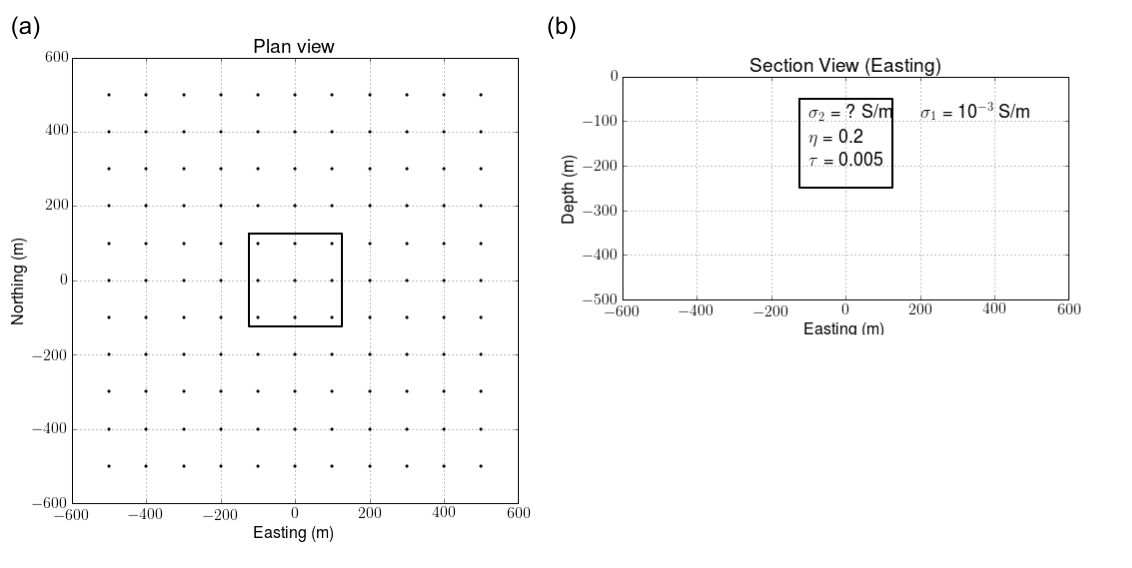
\includegraphics[width=1.0\textwidth]{figures/IPModel.png}
  \caption{Plan (a) and section b) views of the IP model. Dashed line in (a) contours the boundary of the IP body. Solid circles in (a) denotes the location of stations.}
  \label{F: IPModel}
\end{figure}
\clearpage

%%% ===========================================================================
%%% SUBSECTION
\subsection{IP responses}
IP datum ($\dip$) is defined in equation (\ref{eq: IPdatum_syn}) as a subtraction of the fundamental($d^{F}=F[\siginf]$) response from the observation ($d=F[\sigma(t)]$). 
We compute both observation and fundamental response then carry out the subtraction to compute IP response. 
Figure \ref{F:Three_IPresp} shows the observed, fundamental, and IP responses at a sounding location above the center of the IP body for (a) canonical, (b) conductive and (c) resistive models.
We present both $b_z$ (left panel) and $\frac{\partial b_z}{\partial t}$ (right panel).
The amplitude of fundamental responses (blue lines) for the conductive case is ~10 times greater than those for two other cases at 0.01 ms. 
Only the observation (black lines) for the conductive case includes negative values (black dashed lines) in late time channels (near 1 ms). 
We identify distinctive deviation of the observed response from the fundamental respone after 1 ms due to the IP effect for both caononical and conductive cases.
However, for the resistive case, the observation and fudamental are almost coincident due to the minor IP effect. 

Considering the IP effect as a polarization charge build-up in the earth provides us some insights.
The polarization charge build-up occurring in the IP body, may have two main phases: charging and discharging.
After turn-off of current in the loop source, the IP current may increase in the charging phase, and decrease in the discharging phase. 
The steady-state of the IP current may not be reached due to the absence of steady-state electric field for inductive source. 
Although, coupling of the EM and IP effect may be complicated in charging phase, we can expect natural separation of these two effects in discharging phase. 
Charging phase must occur in earlier time, and the EM effect at this time may be dominant to IP effect. 
Discharging phase will occur later time, and the IP effect at this time possibly be dominant to EM effect. 
Observed, fundamental and IP responses shown in Figure \ref{F:Three_IPresp} clearly show this natural separation of EM and IP effects in early and late times. 

To divide these two different phases, we choose a time when the amplitude of $\bzip$ has maximum. 
This maximum polarization time, $t^{pol}_{max}$, may correspond to the time when the maximum  charge build-up occurs. 
We marked this time as black dotted lines in Figure \ref{F:Three_IPresp}.
Sign of $\dbzdtip$ on charging and discharging phases are positive and negative, respectively, which correspondingly suggests increase and decreases in the amount of polarization charge in the earth. 
This time occurs near 1 ms for the conductive case, whereas 0.1 ms both canonical and resistive cases. 
Strong EM induction occuring in the conductor may increase the charging time, whereas canonical body or resistor may have minor EM induction effect. 
In discharging phase, IP responses for both $\bzip$ and $\dbzdtip$ have negative sign, which may have some possibility to be observed as negative transients. 
Similar to the fundamental response, the magnitude of the IP response for the conductive case is much greater than those for two other cases. 
This alludes that we have more possibility to observe IP effect from conductive case than two other cases. 
The resistive case might be hard to be observed in reality due to the minor IP response compared to fundamental response. 

For the brevity of the following analyses, we only consider the conductive case where we have much more chance to observe in practice. 
In addition, we set our data type in following analyses as $\bzip$ because of its linear relationship with the IP current through Biot-Savart law. 
Although decaying curves from a sounding location provides fruitful insights about IP response, we have a number of sounding locations in ATEM survey. 
Thus, observing all sounding location at a time channel will provide more information.  
Figure \ref{F:IPresp_Plan} show interpolated map of the observed, fundamental and IP responses at (a) 0.87 ms and (b) 6.7 ms, which are included in charging and discharging times, respectively. 
At 0.87 ms, the fundamental response is dominant in the observation, whereas the IP response is dominant at 6.7 ms.
At 6.7 ms, the observed data near the IP body show negative values. 
By the subtraction process, we can identify IP datum embedded in the observation.
Especially at 0.87 ms, the observation does not include any negative values, which is a signature of the IP effect. 
However, we can recognize the IP responses embedded in the observation with the subtraction (Figure \ref{F:IPresp_Plan}(a)). 
In practice, we cannot obtain the true $\siginf$ thus, the performance of this EM decoupling process may be dependent on time. 
When the relative strength of the IP response to the fundamental response, EM decoupling may show poor performance. 
At 0.1 ms for the conductive case shown in Figure \ref{eq: e_with_eref}(b) is a good example when this can happen. 
However, the performance may be good at certain late time when the magnitude of the IP response is considerable to that of the fundamental response. 
Both 0.87 and 6.7 ms for shown in Figure \ref{F:IPresp_Plan}, can be promising times when the EM coupling may show good performance with reasonable conductivity. 
\begin{figure}[htb]
  \centering
  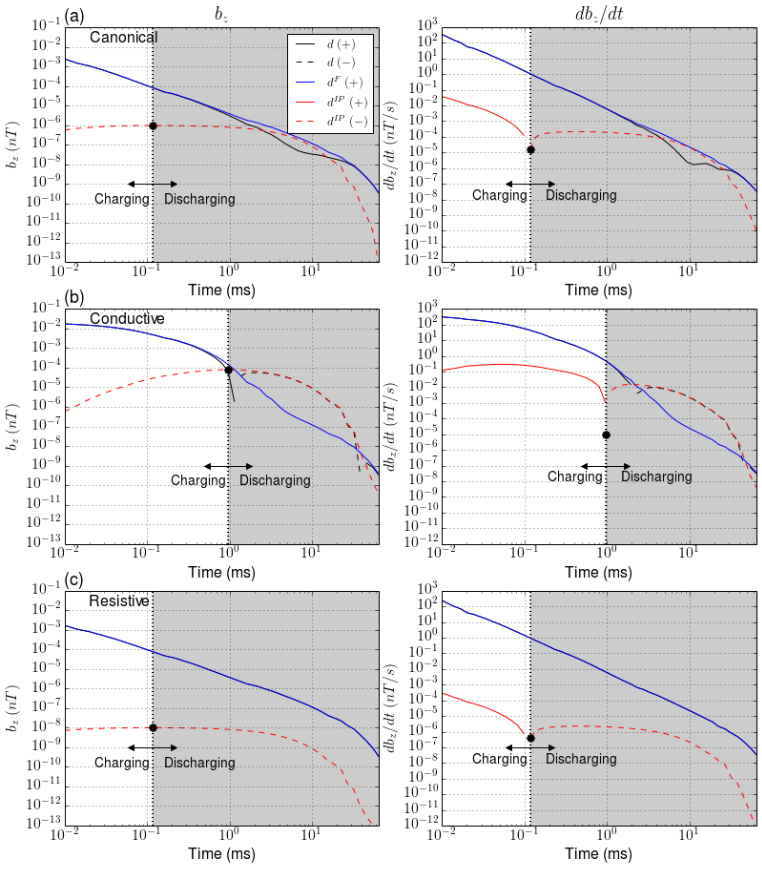
\includegraphics[width=1.\textwidth]{figures/Three_IPresp.png}
  \caption{Time decaying curves of observation ($d$; black line), fundamental ($d^F$; blue line) and IP ($\dip$; red line) responses. All three cases: (a) canonical, (b) conductive and (c) resistive are presented. Right and left panels show $b_z$ and $\frac{\partial b_z}{\partial t}$. Black dotted line indicates the maximum polarization time.}
  \label{F:Three_IPresp}
\end{figure}
\begin{figure}[htb]
  \centering
  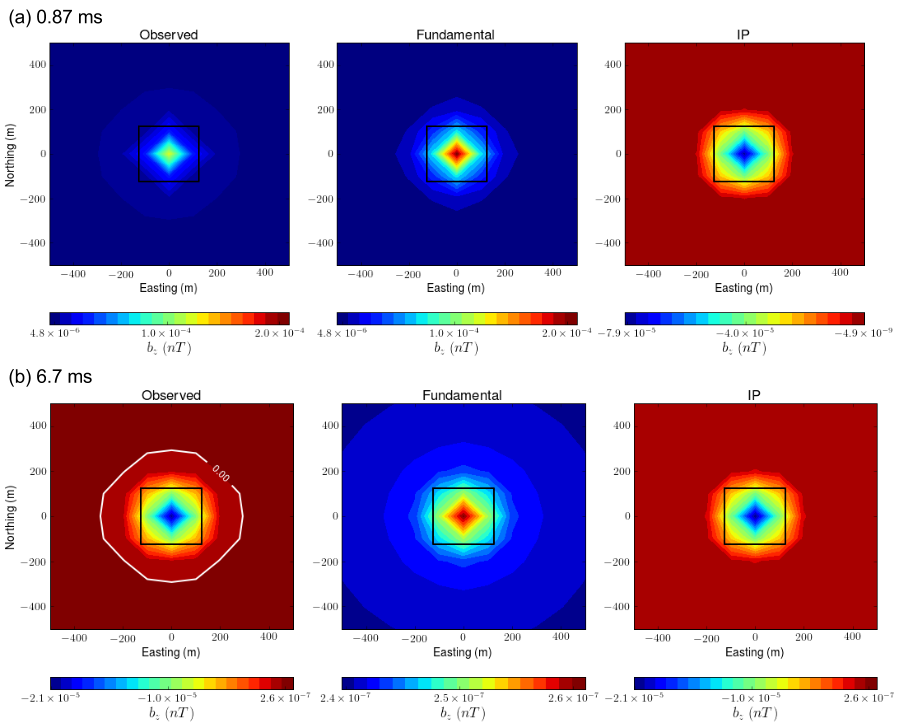
\includegraphics[width=1.\textwidth]{figures/IPresp_Plan.png}
  \caption{Interpolated maps of observed (left panel), fundamental (middle panel) and IP (right panel) responses. Two time channels at (a) 0.87 ms and (b) 6.7 ms are presented. 
  Negative values are blanked as white region.
  }
  \label{F:IPresp_Plan}
\end{figure}
\clearpage

%%% ===========================================================================
%%% SUBSECTION
\subsection{IP currents}
A type of the IP response that we are mainly interested in this study is magnetic flux density ($\b$). 
Thus, the IP response has linear relationship with the IP current as shown in equation (\ref{eq: BiotbIP_approx}).
Careful observation of the total ($\j$), fundamental ($\j^F$) and IP current ($\j^{IP}$) can allow us to understand mechanisms of the IP effect coupled with EM effect. 
Figure \ref{F:IPcurrent_Plan} show those three currents at (a) 0.87 ms and (b) 6.7 ms on plan maps at -125 m-depth. These are the same times that we provide IP responses (Figure \ref{F:Three_IPresp}). 
A transmitter location is denoted as white solid circle in the figure. 
Similar to the IP response, at 0.87 ms in charging phase, the magnitude of the fundamental current is dominant to that of the IP current. 
At 6.7 ms the magnitude of the IP current is dominant to that of the fundamental current, and this time is in discharging phase. 
From the geometric shape of the anomalous currents, we can identify two different type of currents: galvanic and vortex. 
At 0.87 ms, the fundamental current show distortion due to the conductor, and this may correspond to galvanic current. 
On the IP current map, the IP body acts like a dipole, which indicates galvanic current. 
In contrast, at 6.7 ms on the fundamental current map, we observe dominant circulating current in the conductor, which corresponds to the vortex current due to EM induction. 
The IP current map at this time includes both considerable galvanic and vortex currents. 
From the definition of the polarization current (equation (\ref{eq:polarization_current})), the IP current will include time history of the electric field in the IP body through convolution. 
Accordingly, both galvanic and vortex IP currents occurred at 6.7 ms are resulting from both galvanic and inductive effects in the fundamental fields happened at different times. 
We effectively capture both effects into the linearized kernel with a proper choice of the reference electric field shown in equation (\ref{eq:reference_electricfield}). 
Figure \ref{F:Jref_tref} show the reference (a) current and (b) time on plan maps at -125 m-depth. 
Comparison of the reference current and the IP current at 6.7 ms shows that the direction of the IP current is opposite to the reference current. 
Due to the strong EM induction in the conductor, the reference time is greater in the conductor than outside as shown in Figure \ref{F:Jref_tref}(b). 

\begin{figure}[htb]
  \centering
  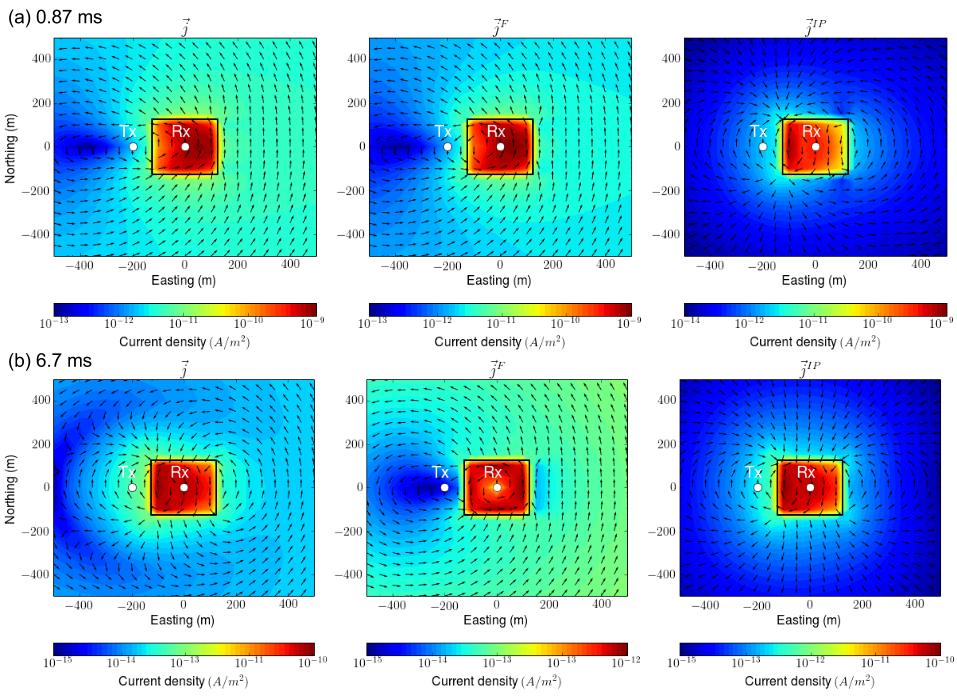
\includegraphics[width=1\textwidth]{figures/IPcurrent_Plan.png}
  \caption{Interpolated maps of total (left panel), fundamental (middle panel) and IP (right panel) currents at -125m-depth. Two time channels at (a) 0.87 ms and (b) 6.7 ms are presented.}
  \label{F:IPcurrent_Plan}
\end{figure}

\begin{figure}[htb]
  \centering
  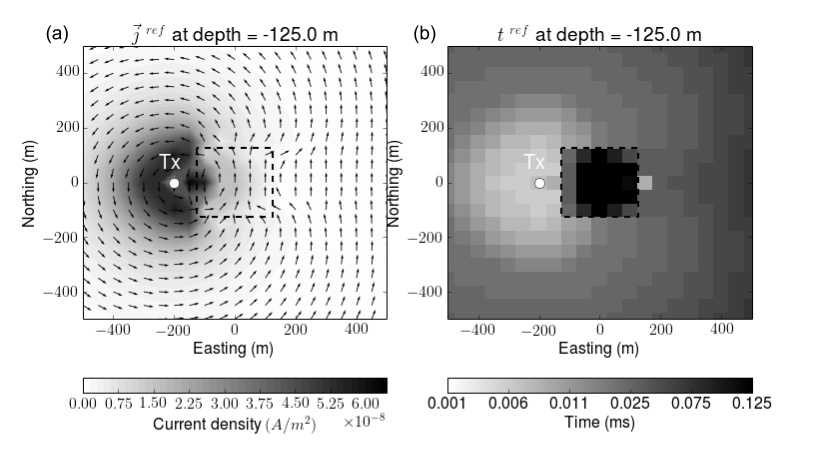
\includegraphics[width=1\textwidth]{figures/Jref_tref.png}
  \caption{Plan view maps of (a) reference current and (b) time for the conductive case at -125m-depth.}
  \label{F:Jref_tref}
\end{figure}
\clearpage

%%% ===========================================================================
%%% SUBSECTION
\subsection{Validation of the linearization}
To derive the linearized kernel for the IP responses, we made some assumptions. 
In this section, by comparing, approximate IP current and responses with true ones, we suggests the reliability of the linearized kernel. 
Similar to the performance of the EM decoupling, in the early time when EM effect is dominant, our linearization may show poor performance. 
This may be mainly caused by ignoring inductive portion of $\e^{IP}$. 
However, we can expect reasonable performance at certain late times when the IP effect is considerable. 
Figure \ref{F:IPcurrent_PlanandSec_late} compares (a) true and (b) approximate IP currents on plan and section view maps at 6.7 ms when the IP effect is considerable to the EM effect. 
Approximate IP current shows good agreement with the true one for both direction and magnitude. 
We apply the Biot-Savart law to both true and approximate IP currents, and compute IP responses. 
To test the reliability of the Biot-Savart law, we also compute IP response by the subtraction of the fundamental response from the observation. 
Figure \ref{F:True_vs_approx_IPresp} show those three IP responses: true IP response from the subtraction ($b_z^{IP}$), true IP response from Biot-Savart law ($b_{z \ BS}^{IP}$), and approximate IP response ($b_{z \ approx}^{IP}$). 
The $b^{IP}_{z \ BS}$ is almost coincident with $\bzip$, which suggests the reliability of the operation for Biot-Savart law. 
The approximate $\bzip$ show reasonable match after 0.2 ms with true one, and converges at it moves to the later time. 
These numerical tests suggest the reliability of our linearization at certain late time channel when the IP effect is considerable to the EM effect. 

\begin{figure}[htb]
  \centering
  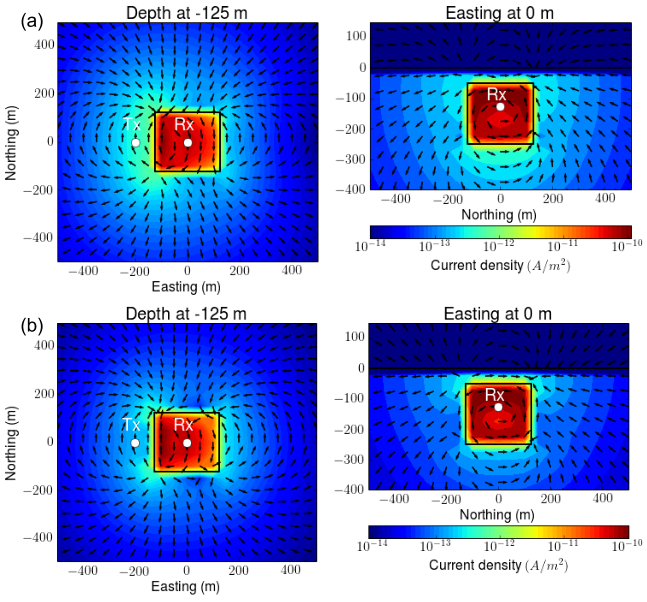
\includegraphics[width=1\textwidth]{figures/IPcurrent_PlanandSec_late.png}
  \caption{Interpolated maps of (a) true and (b) approximate IP currents. Top and bottm panels show plan and section view maps at -125 m-depth and 0m-easting. }
  \label{F:IPcurrent_PlanandSec_late}
\end{figure}

\begin{figure}[htb]
  \centering
  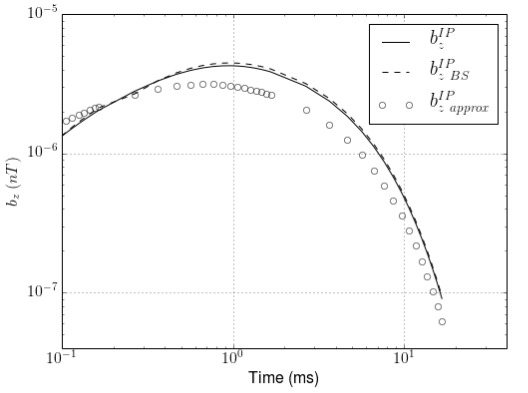
\includegraphics[width=1\textwidth]{figures/True_vs_approx_IPresp.png}
  \caption{Comparison of true and approximate IP respones ($b_z^{IP}$). Solid and dotted lines indicates true $b_z^{IP}$ computed by subtraction process and application of Biot-Savart to true $\j^{IP}$ ($b_{z \ BS}^{IP}$). Empty circles presents approximate $b_z^{IP}$. }
  \label{F:True_vs_approx_IPresp}
\end{figure}
\clearpage

%%% ===========================================================================
%%% SUBSECTION
\subsection{Equivalent pseudo-chargeability}
Validation for the linearized kernel carried out in the previous section is for a sounding location, and this includes evaluation of the pseudo-chargeability. 
The pseudo-chargeability will be different for different sounding locations because $w^e(t)$ will be different. 
For our 3D inversion, we do not recover the pseudo-chargeability for each sounding, but 
recover an equivalent pseudo-chargeability. 
In this section, we test the feasibility of this equivalent pseudo-chargeability. 
For this, we first evaluate $w^e(t)$ and pseudo-chargeability for every sounding, then compose an equivalent pseudo-chargeablity by averaging pseudo-chargeability from some sounding locations, which have major contribution to the IP responses. 

We evaluate $w^e(t)$ for every sounding, and provide $w^e(t)$ at the center pixel of the IP body for four different sounding locations along Easting profile line at 0m-Northing. 
Figure \ref{F:Equivalent_peta}(a) shows $w^e(t)$ from -100m, -200m, -300m and -400m-Easting sounding locations. 
As the sounding location moves away from the center of the IP body, the peak time of the $w^e(t)$ occurs at later time that is, they are not same as we expected. 
Pseudo-chargeability of every sounding location is computed, and we provide those pseudo-chargeability at the same pixel at 6.7 ms in Figure \ref{F:Equivalent_peta}(b). 
Different $w^e(t)$ for each sounding results in different pseudo-chargeability by definition of the pseudo-chargeability in equation (\ref{eq: pseudochargeability}). 
Since this time is after the peak time of $w^e(t)$, the pseudo-chargeability increases as it further away from the center of the IP body. 
From the linearized kernel of IP response (equation (\ref{eq: dIP_lineareq})), we know that the IP response is a dot product of Jacobian matrix and pseudo-chargeability for each sounding. 
Accordingly, contribution of the pseudo-chargeability for each sounding will be dependent on the product of pseudo-chargeability and Jacobian matrix. 
Figure \ref{F:Equivalent_peta}(c) show the product between the center element of pseudo-chargeability and the Jacobian matrix (P-J product) for every sounding location at 6.7 ms. 
We choose nine highest sounding locations about P-J product, which may have major contribution to the IP responses, and marked as empty circles in Figure \ref{F:Equivalent_peta}(b) and (c).
Then by arithmetically averaging pseudo-chargeability from those nine sounding locations, we compose an equivalent pseudo-chargeability. 
Finally, we compute approximate IP responses using this equivalent pseudo-chargeability at 6.7 ms. 
Figure \ref{F:EquivPeta_True_Approx}show the comparison of true and approximate IP responses on plan view map. 
The approximate IP responses evaluated with the equivalent pseudo-chargeability show good agreement with true ones about both the magnitude and geometric shape.
These tests provide that the validity of recovering an equivalent pseudo-chargeability from 3D IP inversion. 

\begin{figure}[htb]
  \centering
  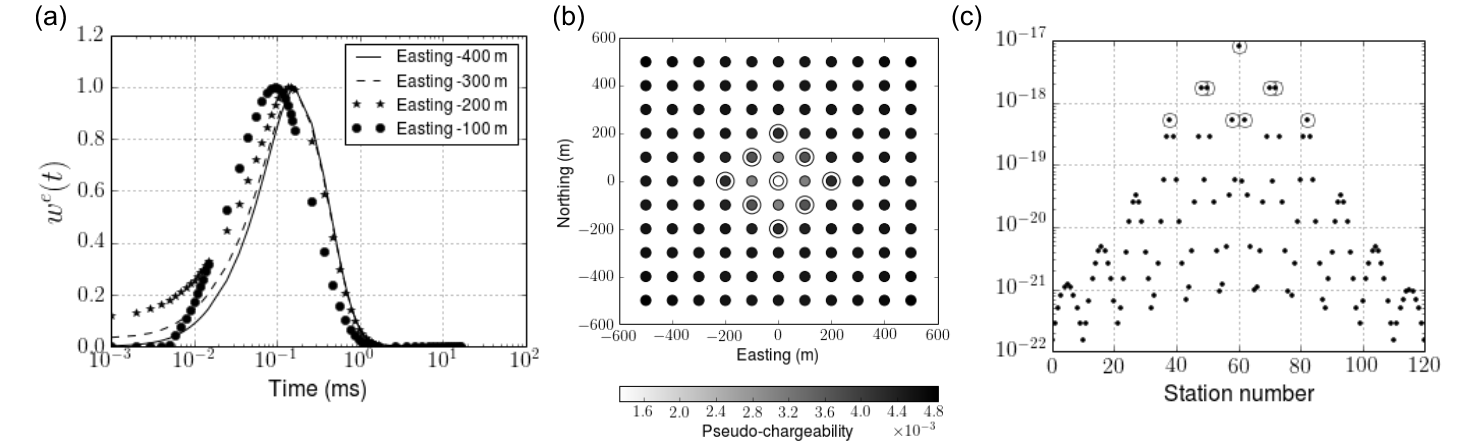
\includegraphics[width=1.\textwidth]{figures/Equivalent_peta.png}
  \caption{(a) The normalized time history of the electric field ($w^e(t)$) at the center pixel of the IP body. Solid lines, dashed lines, stars and solid circles indicate four different transmitters located at Easting -400, -300, -200 and -100 m  along the profile line at 0 m-northing.
  (b) Pseudo-chargeability on the center pixel of the IP body at 7.08 ms for all soundings.
  (c) Pseudo-chargeability and Jacobian (P-J) product at the center pixel of the IP body (6.7 ms) for all soundings.
  }
  \label{F:Equivalent_peta}
\end{figure}

\begin{figure}[htb]
  \centering
  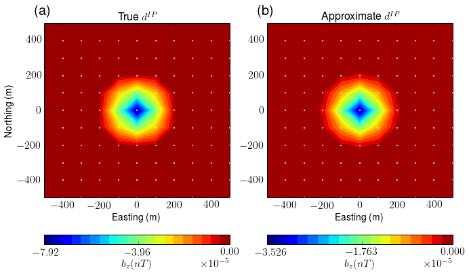
\includegraphics[width=1.\textwidth]{figures/EquivPeta_True_Approx.png}
  \caption{Comparison of (a) true and (b) approximate $b_z^{IP}$ responses at 6.7 ms on plan view map.}
  \label{F:EquivPeta_True_Approx}
\end{figure}

%%% ===========================================================================
%%% SUBSECTION
\subsection{3D IP inversions}
Based on the systematic validation that we have performed in previous sections, we can proceed 3D IP inversion with the linearized kernel.
We apply this inversion to each time channel of the IP datum, and recover multiple times of the pseudo-chargeability. 
Our 3D inversion is based upon \cite{doug1994,Li2000}, and it requires some choices of the inversion paramters. 
Table \ref{table:inversion_params} shows our choices for the inversion parameters, and those are fixed in following inversion examples. 
Because we invert each time channel of IP datum, seprately, the number of the data in the inversion is same as the number of soundings. 
For the trade-off parameter, $\beta$, we first compute initital guess as shown in Table \ref{table:inversion_params}, then decrease the amplitude of $\beta$ with constant rate. 
Each beta iteration can include several inner iterations. 
For the uncertainty, we only used floor value, which is one percent of the maxmimum amplitude of the observed data for every sounding. 
There are two important parameters the Table \ref{table:inversion_params} does not includes: depth weight and positivity constraint. 
These two items will be investigated with numerical examples. 

\begin{table}[ht]
  \caption{Parameters used in 3D IP inversion.} % title of Table
  \centering % used for centering table
  \begin{tabular}{c c} % centered columns (4 columns)
  \hline\hline %inserts double horizontal lines
  Inversion parameters & Value \\
  [0.1ex] % inserts table
  \hline
  The number of data &    11$\times$11=121 \\
  The number of models &  41$\times$41$\times$20=33620 \\
  $\alpha_s$ &  $10^{-5}$\\
  $\alpha_x$ &  1\\
  $\alpha_y$ &  1\\
  $\alpha_z$ &  1\\
  Initial $\beta$ &  $10^{1.5}$ $\frac{\mathbf{x}^T\mathbf{J}^T\mathbf{J}\mathbf{x}}{\mathbf{x}^T\mathbf{W}_m^T\mathbf{W}_m\mathbf{x}}$\\
  Decrease rate of $\beta$ &  0.5\\
  The number of inner $\beta$ iteration & 1\\
  $\mathbf{m}_{ref}$ & $\mathbf{0}$ \\
  Uncertainty & $\epsilon_j$=0.01$\times$max($|\mathbf{d}^{obs}|$) \\
  \hline %inserts single line
  \end{tabular}
  \label{table:inversion_params} % is used to refer this table in the text
\end{table}


%%% ===========================================================================
\subsubsection{Depth weight}
From the linearized kernel shown in equation \ref{eq: dIP_lineareq}, we recognize that all the time dependency in IP datum is originated from the pseudo-chargeability ($\peta(t)$). 
In addition, we invert each time of the IP data, separately. 
Thus, our inversion may not have intrinsic depth resolution, but may have relative depth resolution similar to magnetic inversion (CITEdougmag). 
This indicates that our inversion may require the depth weight. 
For this, we generated IP response at a single time using the linearized kernel by assuming the magnitude of the pseudo-chargeability in the IP body as 1, and that in outside as 0. 
Figure \ref{F:Depthweight}(a) shows the recovered pseudo-chargeability without depth weighting. 
Anomalous pseudo-chargeability is limited to the near surface due to the higher sensitivity on the region, and magnitude of the pseudo-chargeability is underestimated. 
By using the depth weighting shown in equation \ref{eq: weight_mat}, we can image the IP body on the deeper location, which is closer to the true one. 
The magnitude of the recovered pseudo-chargeability ($\sim$0.5) is closer to the true one than the above result without depth weighting. 
Based on this analysis, we use the same depth weighting for following examples. 

\begin{figure}[htb]
  \centering
  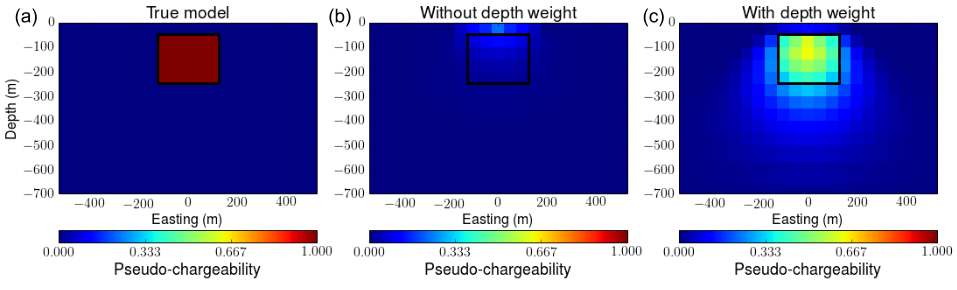
\includegraphics[width=1.\textwidth]{figures/Depthweight.png}
  \caption{Effect of depth weight in 3D IP inversion. (a) True pseudo-chargeability model on vertical section at 0 m-northing. Recovered pseudo-chargeability models (b) without depth weight and (c) with depth weight.}
  \label{F:Depthweight}
\end{figure}
\clearpage

%%% ===========================================================================
\subsubsection{Incorrect conductivity}
We compute IP datum by subtracting fundamental response from the observation. 
However, evaluation of the fundamental response requires the true $\siginf$. 
Because we cannot obtain true $\siginf$ in 3D, computed IP datum from the subtraction process shown in equation \ref{eq: IPdatum_syn} may include some residual field. 
To observe the effect of this residual field in the 3D IP inversion, we perturbed conductivity of the half-space ($\sigma_1=0.001$ S/m) as two times larger and smaller with the the true $\sigma_2$ (0.01 S/m).

Using two perturbed $\siginf$ models and the true $\siginf$ model, we computed fundamental responses, and subtract those from the observation. 
Figure \ref{F:Reg_IPresp} show those three IP responses of a profile line at 0m-Northing at 1 ms.  
When the half-space conductivity is greater than true one ($2\times\sigma_1$), we overestimate IP datum that is, it contains negative residual field. 
Similarly, we underestimate IP datum when the half-space conductivity is smaller than the true one ($0.5\times\sigma_1$) thus, the IP datum includes positive residual field.
We invert these three IP responses, and provide sections of the recovered pseudo-chargeability at 0m-Northing. 
Figure \ref{F:Regional_IPInv}(a), (b) and (c) correspondingly show the recovered pseudo-chargeability from true, overestimated, and underestimated IP responses. 
With the true IP response, geometry of the IP body is reasonably recovered. 
Due to the negative residual field, the recovered pseudo-chargeability from the overestimated IP responses show positive-valued artifacts near the IP body (Figure \ref{F:Regional_IPInv}(b)). 
In contrast, when the IP datum includes positive residual field, we have negative-valued artifacts near the IP body (Figure \ref{F:Regional_IPInv}(c)) . 
Based on the definition of the  $w^e{t}$ and pseudo-chargeability and shown in equations \ref{eq: we} and \ref{eq: pseudochargeability}, the sign of the pseudo-chargeability should be positive. 
We can use this information as a positivity constraint in the inversion as shown in equation \ref{eq10}. 
Recovered pseudo-chargeability with this constraint for the underestimated case is shown in Figure \ref{F:Regional_IPInv}(d). 
Due to the positivity constraint, the inversion excludes to have negative values in the recovered pseudo-chargeability. 
Comparison of the observed and predicted data for this case shown in Figure \ref{F:Reg_obspred} clearly shows how this constraint prevents not to fit the positive residual fields originated from underestimated conductivity. 
We use this constraint for following examples. 

To compute the sensitivity function, we need the reference electric field, which is dependent on conductivity. 
Therefore, the incorrect conductivity will have an effect on the sensitivity function as well. 
In order to test this effect, we compute Jacobian matrix using canonical model (true half-space model). 
Figure \ref{F:True_vs_approx_sensitivity} compares the recovered pseudo-chargeability from the 3D IP inversion of the IP datum at 1.0 ms with the true and incorrect sensitivity function using half-space conductivity. 
Both recovered models does not show significant difference, which suggests robustness of our sensitivity function about the incorrect conductivity. 
This implies that even we do not have 3D conductivity model, one can still apply our 3D IP inversion using half-space conductivity if the ATEM data includes distinctive negative response. 

\begin{figure}[htb]
  \centering
  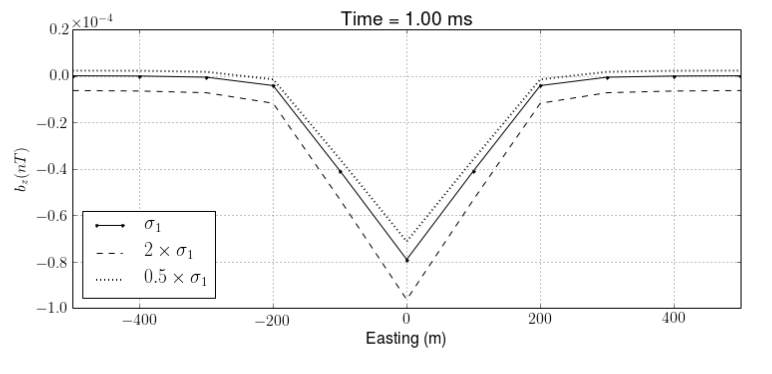
\includegraphics[width=1.\textwidth]{figures/Reg_IPresp.png}
  \caption{IP responses on a profile line at 0 m-northing. Overestimated and underestimated $\dip$ responses are computed from perturbed $\siginf$ models. Half-space conductivity ($\sigma_1$) is perturbed two times higher or less. Dotted and dashed lines show $\dip$ responses from $2 \times \sigma_1$ and $0.5 \times \sigma_1$, respectively. Solid lind show the true $\dip$ response. }
  \label{F:Reg_IPresp}
\end{figure}

\begin{figure}[htb]
  \centering
  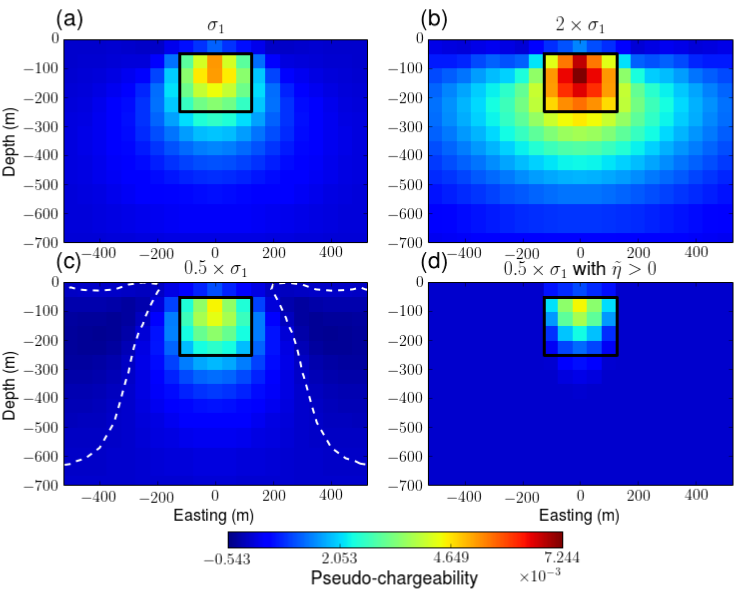
\includegraphics[width=1.\textwidth]{figures/Regional_IPInv.png}
  \caption{Recovered pseudo-chargeability sections from 3D IP inversions at 0 m-northing. (a) $\dip$ with true $\sigma_1$. (b) $\dip$ with 2$\times \sigma_1$. (c) $\dip$ with 0.5$\times \sigma_1$. (d) $\dip$ with 0.5$\times \sigma_1$ and the positivity constraint on the pseudo-chargeability.}
  \label{F:Regional_IPInv}
\end{figure}

\begin{figure}[htb]
  \centering
  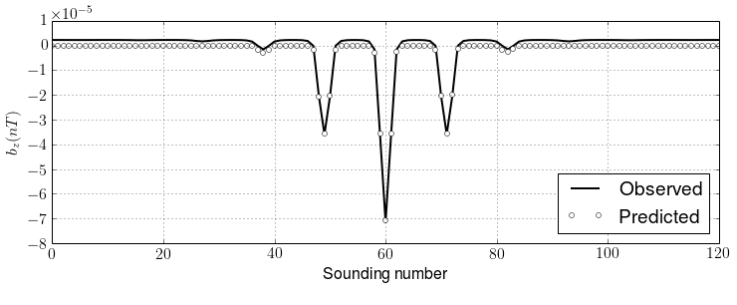
\includegraphics[width=1.\textwidth]{figures/Reg_obspred.png}
  \caption{Comparison of the observed (solid line) and predicted (empty circles) data. $\dip$ response was generated with underestimated half-space condutivity (0.5$\times \sigma_1$). The positivity constraint was used the 3D IP inversion.}
  \label{F:Reg_obspred}
\end{figure}

\begin{figure}[htb]
  \centering
  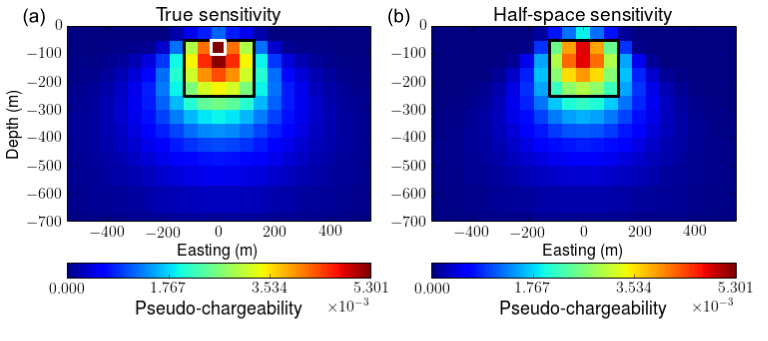
\includegraphics[width=1.\textwidth]{figures/True_vs_approx_sensitivity.png}
  \caption{Recovered pseudo-chargeabilty sections from the 3D IP inversions at 0m-northing.  (a) True and (b) incorrect $\siginf$ is used to compute sensitivity function. For the incorrect sensitivity we used half-space conductivity ($\sigma_1$).}
  \label{F:True_vs_approx_sensitivity}
\end{figure}
\clearpage

%%% ===========================================================================
\subsubsection{Extracting intrinsic IP parameters}
Although we recovered 3D pseudo-chargeability from the ATEM data, which provides distribution of chargeable bodies in the earth, still the pseudo-chargeability is not the intrinsic IP  parameters like the chargeability and time constant.
Fortunately, we have some possibility to recover this intrinsic IP information by interpreting multiple times of pseudo-chargeability together as we explained section \ref{section: extract_intrinsicIP}. 
We separately apply 3D IP inversion to the multiple channels of the IP datum ranging from 1-10 ms (14 channels), and recover pseudo-chargeability at those times. 
Here we choose true $\siginf$ model for both evaluation of IP datum and sensitivity function. 
To test the possibility of extracting intrinsic parameters from those recovered pseudo-chargeability at multiple times, we first choose a single pixel in the IP body shown in Figure \ref{F:IntrinsicIP}(a).  
This can be considered as the data for the inverse problem that we are going to solve to  estimate time constant ($\tau$) and chargeability ($\eta$) assuming $c$=1. 
A forward kernel for this inversion is shown in equation \ref{eq: pseudochargeability_petaI}. 
Averaged $w^e(t)$ from nine sounding locations chosen in Figure \ref{F:Equivalent_peta}(b) at the selected pixel of in the IP body is shown in Figure \ref{F:IntrinsicIP}(a).
The selected pixel is marked as white rectangle in Figure \ref{F:True_vs_approx_sensitivity}(a).  
Time decays of the observed and predicted data are shown in Figure \ref{F:IntrinsicIP}(b).
The estimated time constant ($\tau_{est}$) and chargeability ($\eta_{est}$) are 0.005 and 0.08, respectively. 
These are reasonable compared the those for true ones: 0.005 and 0.1, which suggests a potential to extract intrinsic IP parameters from ATEM data. 

\begin{figure}[htb]
  \centering
  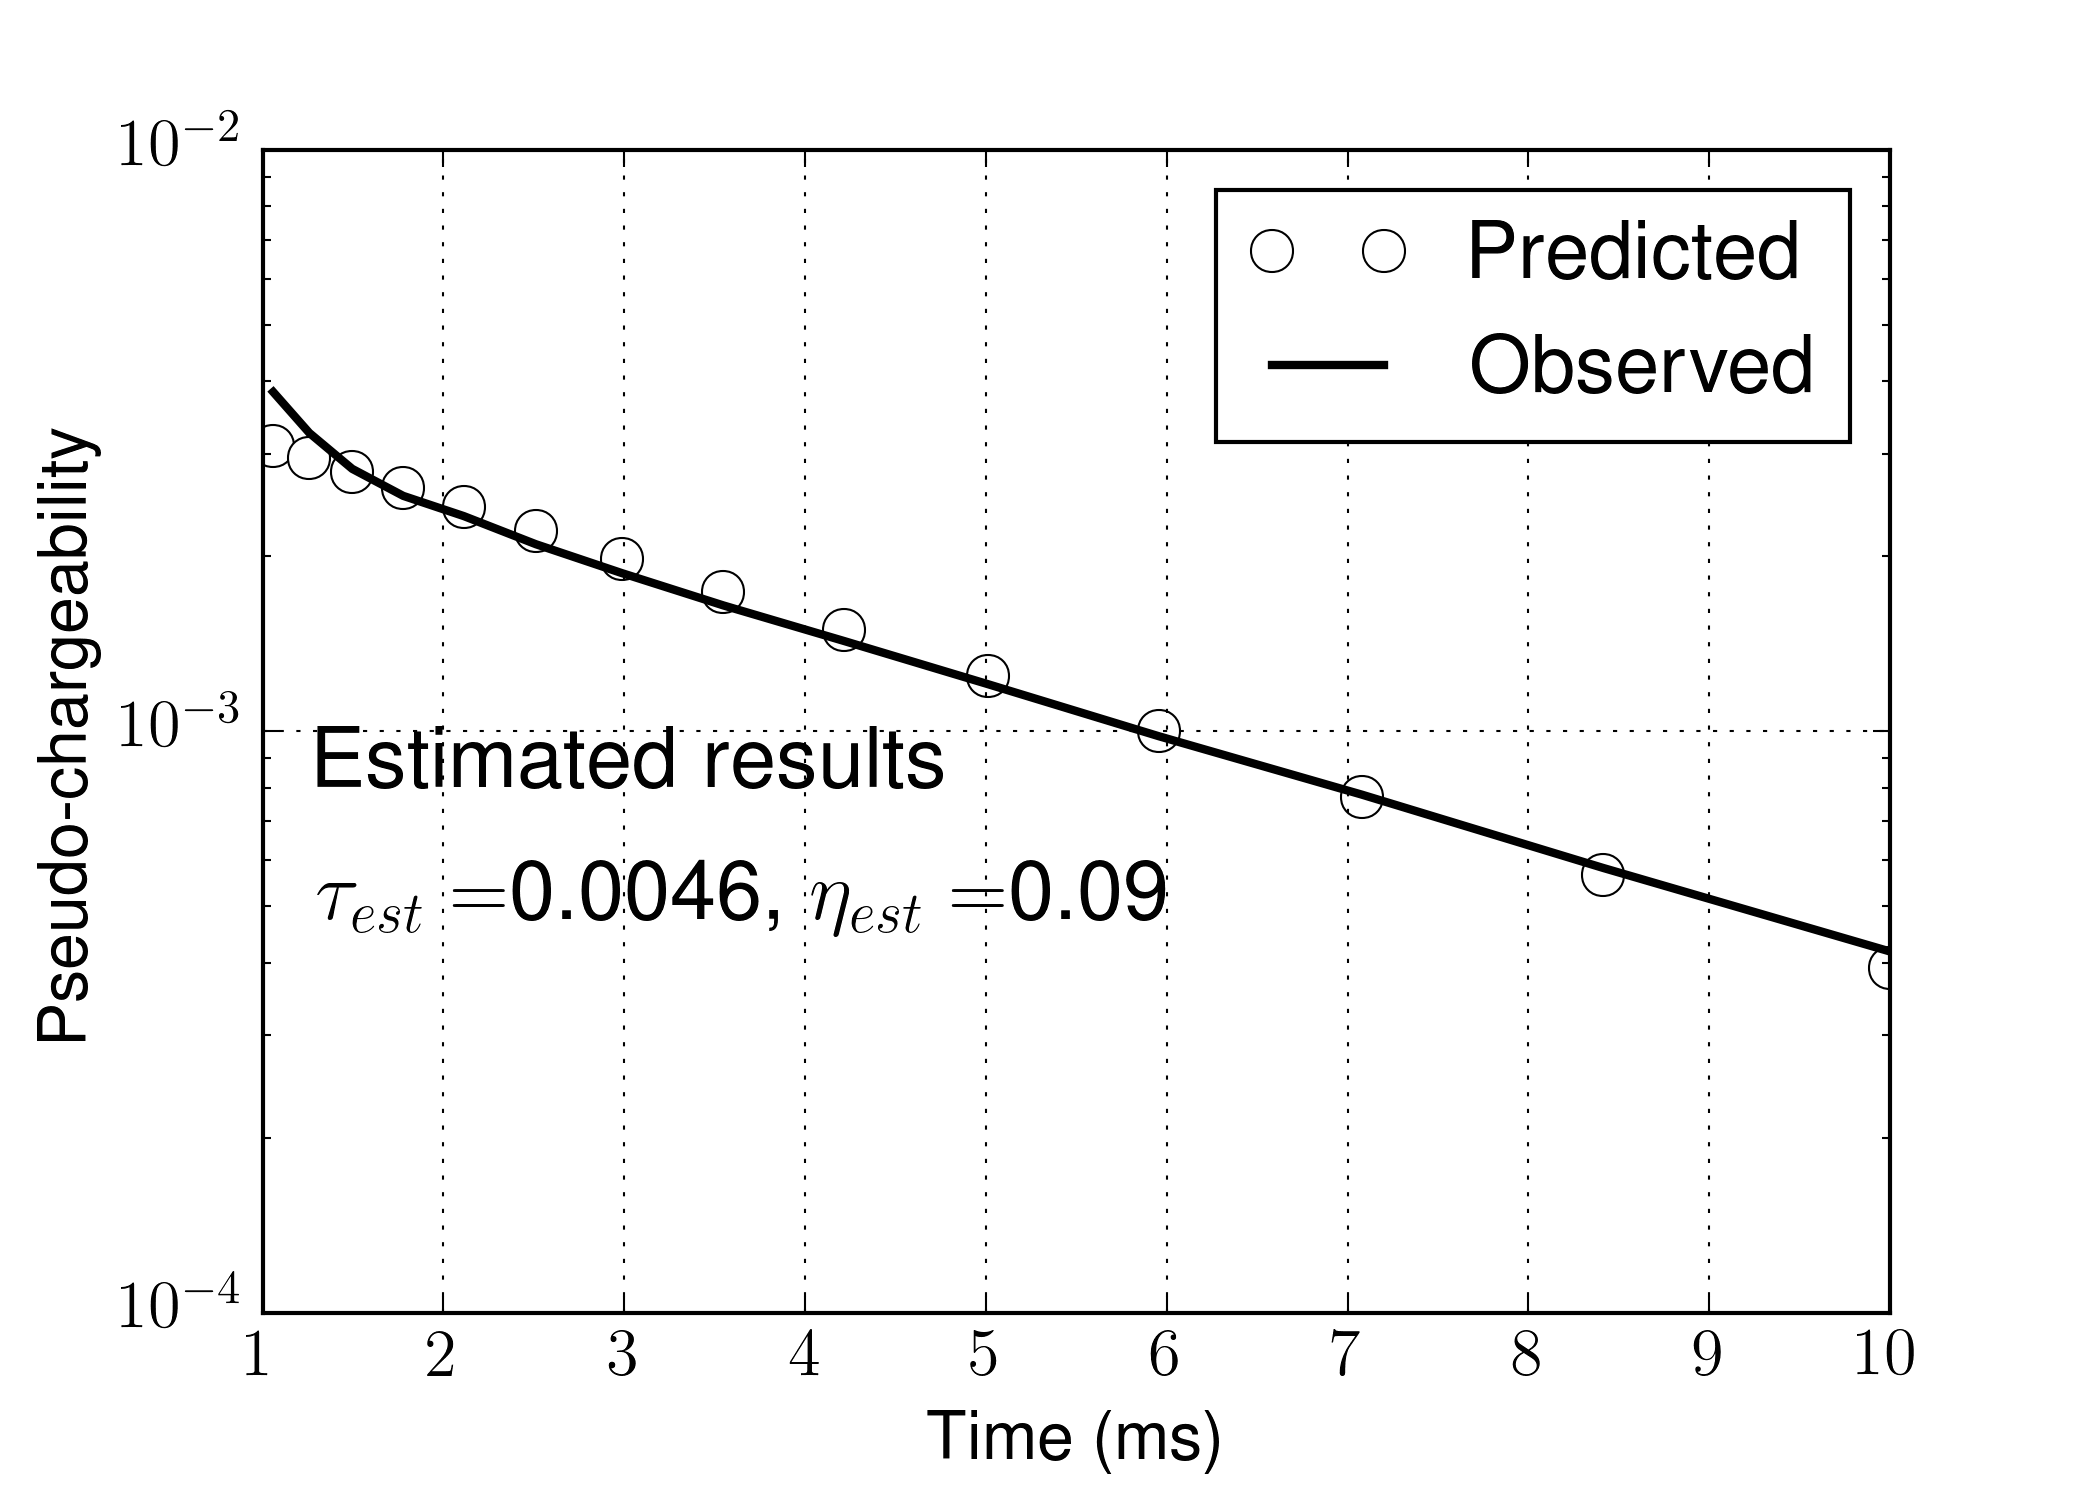
\includegraphics[width=1.\textwidth]{figures/IntrinsicIP.png}
  \caption{(a) The averaged $w^e(t)$ at the single pixel in the IP body (marked as white lines in \ref{F:True_vs_approx_sensitivity}(a). 
  (b) Comparisons of the observed (line) and predicted (empty circles) pseudo-chargeability at the same pixel. Estimated time constant and chargeability are expressed as $\tau_{est}$ and $\eta_{est}$, respectively.}
  \label{F:IntrinsicIP}
\end{figure}
\clearpage

%% =============================================================================
%% Section. Discussions
%% =============================================================================

\section{Discussions}
Our linearized kernel for the conductive case showed good performance at certain late time when the IP effect is considerable to the EM effect. 
In the section \ref{section: numerical_examples}, we only showed conductive case to test our linearized kernel to make this article concise. 
However, the capability of the linearization may be different for different conductivity structures. 
To briefly treat this point, we consider the main assumption that we have made in equation (\ref{eq: eip_approx}). 
Here we ignored inductive portion ($\vec{a}^{IP}$) in the $\e^{IP}$. 
We evaluate this assumption by applying Helmholtz decomposition shown in equation (\ref{eq: eip_helmholtz}). 
Detailed description of the evaluation of this decomposition in discrete space is treated in section \ref{section:helmholtz}. 
Based on this, the IP current can be written as
\begin{equation}
  \j^{IP} = \j^{pol}-\siginf \grad \phi^{IP}-\siginf \vec{a}^{IP}.
\end{equation}
If the second term is minor, then our linearization may show good performance. 
Figure \ref{F:IPcurrents_helmholtz} show these three currents: $\j^{pol}$, $-\grad\phi^{IP}$, and $-\siginf\vec{a}^{IP}$ at 6.7 ms for (a) canonical, (b) conductive, and (c) resistive cases. 
The polarization current is the dominant term for all three cases in the IP current. 
For all three cases, the third term ($\siginf\vec{a}^{IP}$) associated with the inductive portion of $\e^{IP}$ is minor, which suggests the reliability of our assumption. 

On top of that, we have tested canonical and resistive cases with the same validation procedures for the conductive case, and summarized the performance of the linearization for each case in Table \ref{table:summary}. 
In the Table \ref{table:summary}, we classified performance as the early and late times. 
The early time indicates the time when the EM effect is dominant, and this time likely be included in charging time. 
The late time indicates the time when the IP effect is considerable to the EM effect, and this time possibly be occurring in discharging time.
All three cases show good performance in the late time.
Even at the early time, canonical and resistive cases show good performances. 
These results provide the capability of our approach for different conductivity structures. 

\begin{figure}[htb]
  \centering
  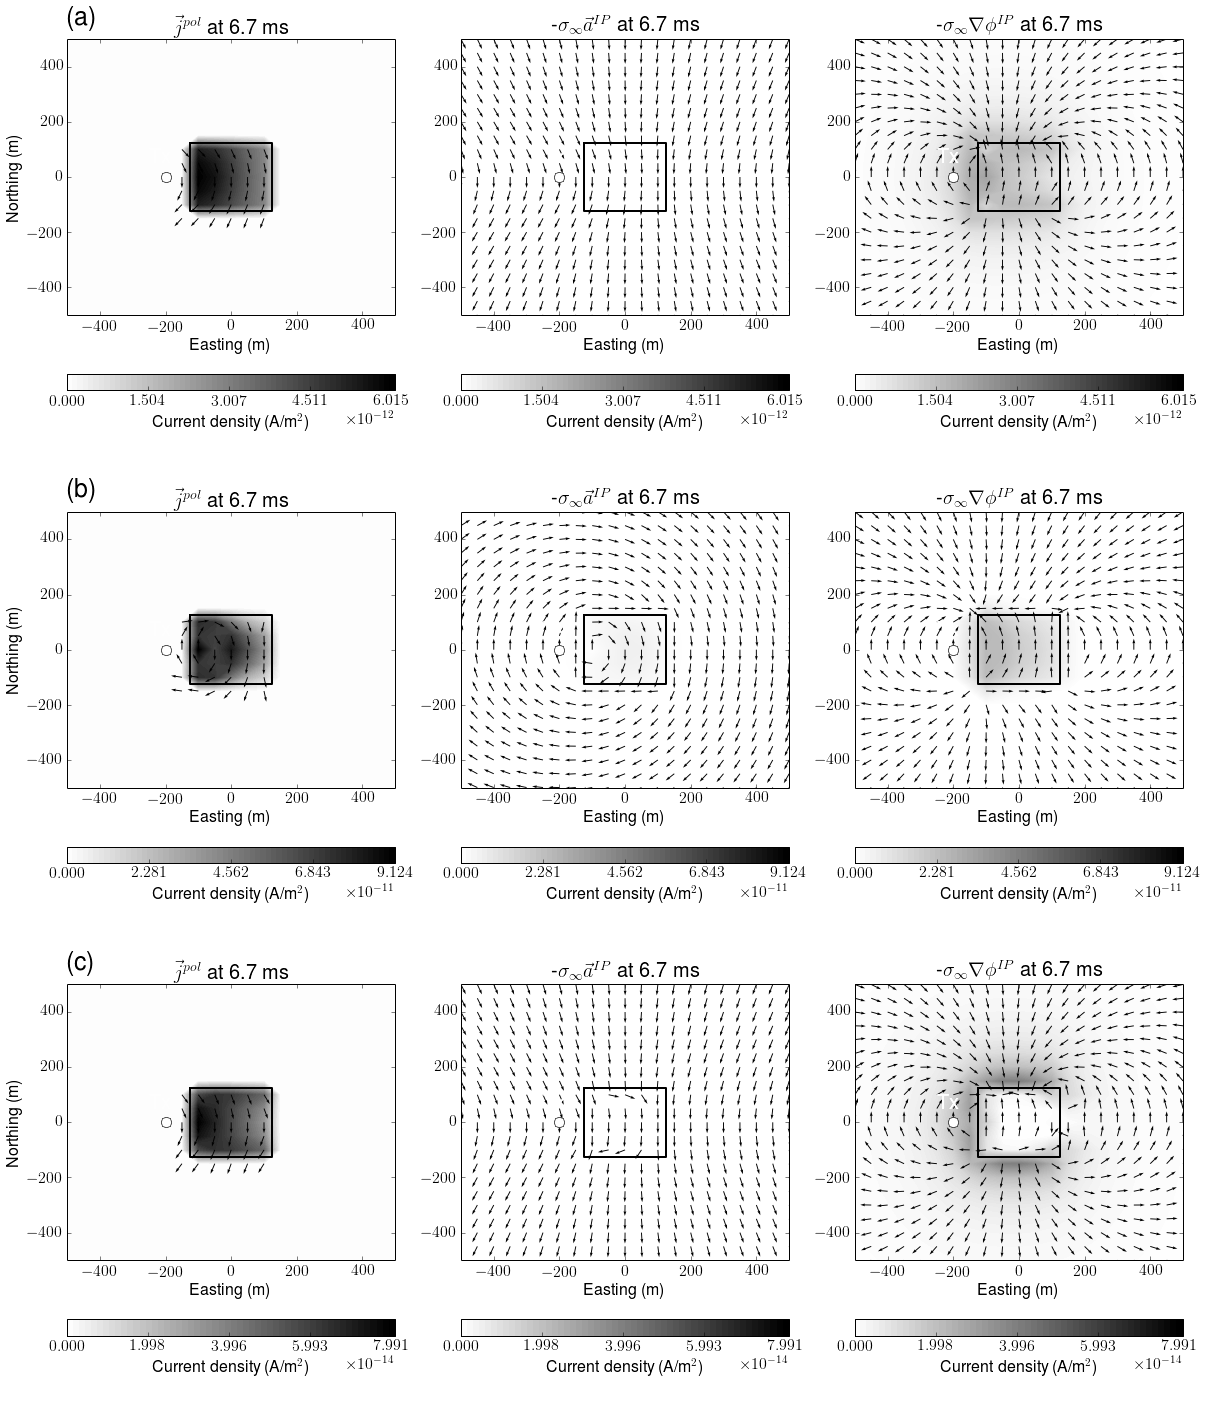
\includegraphics[width=1.\textwidth]{figures/IPcurrents_helmholtz.png}
  \caption{Decomposition of the IP currents as $\j^{pol}$ (left panel), $-\siginf\vec{a}^{IP}$ (middle panel), and $-\siginf\grad\phi^{IP}$ (right panel). Plan view maps of the currents at -125 m-depth are shown. (a) Canonical, (b) Conductive, and (c) Resistive cases. }
  \label{F:IPcurrents_helmholtz}
\end{figure}

\begin{table}
 \caption{Summary of the performance of thel linearized kernel.}
 \label{table:summary}
 \centering
 \begin{tabular}{@{}lccc}
  Division & Case1 & Case2 & Case3  \\
  \hline
  Early & good & poor & good  \\
  Late & good & good & good \\
 \end{tabular}
\end{table}
\clearpage

%% =============================================================================
%% Section. Conclusions
%% =============================================================================
\section{Conclusions}
In this paper, we have introduced an IP inversion procedure for the inductive source TEM data. 
This includes three main steps: 1) subtraction of the fundamental response from the observation, 2) linearization of the IP response as a function of the pseudo-chargeability, and 3) restoration of 3D pseudo-chargeability at multiple times, and further interpretation of the pseudo-chargeability to extract intrinsic IP parameters like Cole-Cole model. We used ATEM survey to test our IP inversion procedure.

Assuming that we can recover reasonable 3D conductivity by inverting TEM data with exception of the IP-contaminated data, evaluation of the first step allows us to identify IP responses embedded in the observation. 
By taking analogy from the EIP case, we effectively linearize ISIP response in time domain as a function of the pseudo-chargeability. 
This pseudo-chargeability was defined as a fraction of the polarization current and the reference current, which may provide us the strength of the IP effect. 
Different from the EIP case, the polarization charge build-up does not reach to the steady-state for the ISIP case due to the absence of steady-state electric field for inductive source. 
This fundamental difference is carefully incorporated to the linearization with a proper choice of the reference electric field. 
Numerical tests on the approximate IP current and responses demonstrated the capability of the linearized kernel for various conductivity structures: canonical, conductive, and resistive cases. 
Our linearization is effective at certain late time when the IP effect is considerable to the EM effect, which may occur in the discharging phase. 

In order to formulate 3D IP inversion, we suggested an equivalent pseudo-chargeability, which represents pseudo-chargeability of every transmitter, and tested with numerical simulation. 
Based on this, we inverted IP responses at multiple times, separately, and recovered pseudo-chargeability at those times.
Due to the lack of intrinsic depth resolution in our kernel, the depth weight is used to locate the chargeable body in the earth. 
3D IP inversion recovered reasonable geometric shape and location of the chargeable body. 
Because we may not recover true conductivity in practice, we tested possible effects of incorrect conductivity. 
Two important places where we use conductivity are EM decoupling and sensitivity functions. 
By designing two situations where we have postive and negative residual field in the IP response, we investigated the effect of incorrect conductivity in the IP response and the inversion. 
For the positive residual fields, we showed that positivity constraint can be effectively used to prevent fitting those residual fields. 
In addition, we recovered important information of chargeable body such as geometric shape and location even with a sensitivity function computed using half-space conductivity model. 
Finally, by interpreting recovered pseudo-chargeability at the center pixel of the IP body in time, we extracted Cole-Cole parameters: $\tau$ and $\eta$ by assuming $c=1$. 
Estimated $\tau$ and $\eta$ were close to true ones, which indicates a potential to recover intrinsic IP parameters from TEM data.  

Our IP inversion procedure provides a framework that one can recover 3D distribution of the pseudo-chargeability, and possibly extraction of intrinsic IP parameters with post-processings of the pseudo-chargeability. 
Because our inversion procedure requires 3D distribution of $\siginf$, which may not be trivial in some cases, this should be carefully investigated in the future for practical application of our inversion methodology. 
In addition, our numerical examples was only treated the ATEM survey, even though application to different types of inductive source TEM survey such as Large-loop TEM may have different aspects that we need to consider. 
However, still important items including EM decoupling, linearization and 3D IP inversion, which have been come up with and carefully tested in this study will be fundamental backgrounds of following studies about the ISIP in time domain. 

% =======================================================================
% SECTION (Appendix)
% =======================================================================

\section{Appendix}
%%% ===========================================================================
%%% SUBSECTION
\subsection{Discretization of steady-state Maxwell's equations}
\label{section:maxwell_discrete}
As shwon equation (\ref{eq: phiIPapprox_general}), computation of our linearized kernel requires solving steady-state Maxwell's equations. 
We discretize this system using mimetic finite volume (FV) method with weak formulation (\cite{Eldadbook}). 
For the discretization, we assume that the electric field $\e$ is discretized by grid function $\de$ on cell edges and magnetic flux density $\b$ is discretized by grid fuction $\db$ on cell faces. 
Electrical potential $\phi$ is discretized by grid fucntion  $\phi$ on cell nodes. For clear representation of the derivation, recall Maxwell's equations in steady state as
\begin{align}
  \j = \siginf\e = -\siginf\grad \phi, \\
  -\div \j = \div \j_s, \\
  \j\big|_{\partial \Omega}\cdot\hat{n} = 0,
  \label{eq:DCBCneumann}
\end{align}
where $\partial \Omega$ indicates boundary surface of the system and $\hat{n}$ is the normal vector of the boundary surface. Weak form of those equations can be written as
\begin{align}
  (\j, \vec{w}) + (\siginf \grad \phi, \vec{w}) = 0, \\
  -(\j, \grad \psi) = (\j_s, \grad \psi).
\end{align}
The inner products $(\j, \vec{w})$, $(\siginf \grad \phi, \vec{w})$,  $(\j, \grad \psi)$ and $(\j_s, \grad \psi)$ are edge based products. Here we define the inner product as
\begin{equation}
  (\vec{a}, \vec{b}) = \int_{\Omega} \vec{a}\cdot\vec{b} dv,
\end{equation}
where $\Omega$ is the volume of the system. By discretizing $\grad$ operator and the inner product in space, we obtain
\begin{equation}
  \Me\dj + \MeSigInf\dgrad\boldsymbol{\phi} = 0,
  \label{eq:DCdisceq1}
\end{equation}
\begin{equation}
  -\dgrad^T \Me\dj = \dgrad^T \Me\dj_s,
  \label{eq:DCdisceq2}
\end{equation}
where $\mathbf{M}^e_i$ is the mass matrices, which discretize the edge based inner product (\cite{Eldadbook}). This inner products are defined  as
\begin{align}
  \mathbf{M}^e_i = \diag(\Ace^T\diag(\vol)\mathbf{i}).
\end{align}
Here, $\mathbf{i}$ indicates a grid function on cell center like $\siginf$, and $\vol$ is the grid function for the cell volume. The averaging matrix $\Ace$ averages discrete function defined on the edges to the cell center. The mass matrix $\Me$ without subscript $i$ indicates that $\mathbf{i}$ is equal to the identity column vector of which all elements are one. By substituting equation (\ref{eq:DCdisceq1}) to (\ref{eq:DCdisceq2}), we have
\begin{equation}
  \A_{\siginf}\boldsymbol{\phi} = \mathbf{rhs}^{DC},
  \label{eq:DCdiscLin}
\end{equation}
where $\A_{\siginf} = \dgrad^T \MeSigInf\dgrad$ and $\mathbf{rhs}^{DC} = \dgrad^T \Me\dj_s$. 

%%% ===========================================================================
%%% SUBSECTION
\subsection{Discretization of the linearized kernel}
\label{section:linearkernel_discrete}
To obtain linear form of equation shown in equation (\ref{eq: dIP_lineareq}),
we first discretize Biot-Savart law shown in equations (\ref{eq: BiotbIP_approx}) and (\ref{eq: BiotbIPdt_approx}). In our discretization $\j^{IP}$ and  $\peta$ are defined on the cell center, and those for each time channel are constant in a cell volume, whereas $\eref$ is defined on the cell edges. 
We define the number of cells and edges in 3D space as nC and nE, respectively. Discretized IP current density, $\dj^{IP}_{cc} \in \mathbb{R}^{3nC}_{1}$, and defined on the cell center, since $\j^{IP}$ has three components, we first discretize integration operator including cross product ($\int_{v}\frac{ \times \hat{r}}{r^2}dv$) as
\begin{equation}
  \mathbf{G}_{Biot} =
  \begin{bmatrix}
       \mathbf{e}^T &  \mathbf{0}   & \mathbf{0}  \\
       \mathbf{0}   &  \mathbf{e}^T & \mathbf{0}  \\
       \mathbf{0}   &  \mathbf{0}   & \mathbf{e}^T
    \end{bmatrix}
  \begin{bmatrix}
       \mathbf{0}     &   \mathbf{S}_z   & -\mathbf{S}_y  \\
      -\mathbf{S}_z   &   \mathbf{0}     &  \mathbf{S}_x  \\
       \mathbf{S}_y   &  -\mathbf{S}_x   &  \mathbf{0}
    \end{bmatrix},
 \end{equation}
where
\begin{eqnarray*}
  \mathbf{S}_i =\diag(\mathbf{v}\oplus \mathbf{r}_i \oplus \frac{1}{\mathbf{r}^2}), \ i = x, \ y, \ z
\end{eqnarray*}
and the electric field, $\mathbf{e} \in \mathbb{R}^{nE}_1$ is a column vector, $\diag(\cdot)$ is the diagonal matrix and $\oplus$ is the Hadamard product. 
Then we discretize $\j^{IP}$ shown in equation (\ref{eq: jip_approx}) as
\begin{eqnarray}
  \dj^{IP}_{cc}(t) = \mathbf{S}\diag(\de^{F}_{max})\Ace^T\diag(\vol)\diag(\siginf)\peta(t),
\end{eqnarray}
where
\begin{eqnarray}
  \mathbf{S} = -\mathbf{A}^{e}_{ccv}\Me^{-1}[-\MeSigInf \mathbf{G} \A_{\siginf}^{-1}\mathbf{G}^T + \mathbf{I}] \diag(\de^{F}_{max})\Ace^T\diag(\vol)\diag(\siginf).
\end{eqnarray}
and $\mathbf{A}^{e}_{ccv}$ is discrete averaging matrix from edge to cell center with consideration of three component vector: $\in \mathbb{R}^{3nC}_{nE}$. 
Thus, we can have linear equation for $k^{th}$ time channel as
\begin{eqnarray*}
  \db^{IP}_k = \Gbiot \mathbf{S} \peta_k,
\end{eqnarray*}
where sub-index $k$ indcates $k^{th}$ time channel. Finally, by letting
\begin{equation}
  \mathbf{J} = -\Gbiot\mathbf{S},
  \label{eq: Sense}
\end{equation}
we have
\begin{eqnarray}
  \db^{IP}_k = \mathbf{J}\peta_k,
  \label{eq: bIP_linear}
\end{eqnarray}
where $\mathbf{J}$ is the Jacobian matrix of the linear equation, and since $\mathbf{J}$ is static, we also obtain
\begin{eqnarray}
  -\frac{\partial\db^{IP}_k}{\partial t} = \mathbf{J}(-\frac{\partial \peta}{\partial t}\Big|_k).
  \label{eq: dbIPdt_linear}
\end{eqnarray}

\subsection{Discrete Helmholtz decomposition}
\label{section:helmholtz}
In continuous space, we can decompse arbitrary vector field as 
\begin{equation}
  \e = -\grad\phi -\vec{a},
\end{equation}
where $\div \vec{a} = 0$. 
Decomposition of discrete electric field, $\de$, can be expressed as
\begin{equation}
  \Me\de = -\Me\dgrad \boldsymbol{\phi} -\Me\mathbf{a},
\end{equation}
where $\boldsymbol{\phi}$ and $\mathbf{a}$ are discrete scalar and vector potentials, respectively. 
By taking discrete divergece ($-\dgrad^T$), we obtain
\begin{equation}
  -\dgrad^T\Me\dgrad\boldsymbol{\phi} = \dgrad^T\Me\mathbf{a} + \dgrad^T\Me\de
\end{equation}
Since the vector potential $\vec{a}$ is divergece free, the first term in the right-hand side is zero. Thus, we obtain
\begin{equation}
  \dgrad^T\Me\dgrad\boldsymbol{\phi} = -\dgrad^T\Me\de. 
\end{equation}
By solving this linear system we can first compute $\boldsymbol{\phi}$, then by subtracting this from $\de$, we can also obtain the vector potental, $\mathbf{a}$. 
%%% Appendix
% 1. Discretization of the linearized kernel
% 2. Numerical evaluation of the Helmholtz decomposition

\bibliographystyle{plain}
\bibliography{reference}

\end{document}



